L'existence d'un \ngone\ solution du problème d'isopérimétrie polygonale nécessite un moyen \og continu \fg\ de calculer une aire polygonale, ou plus généralement celle d'un \ncycle.
Pour ce faire, nous utiliserons l'aire algébrique qui est définie pour tout \ncycle\ $\setproba{L} = A_1 A_2 \cdots A_n$ par $\frac12 \dsum_{i=1}^{n} \det \big( \vect{\Omega \primeit{A}_i} , \vect{\Omega \primeit{A}_{i+1}} \big)$ indépendamment du point $\Omega$.%
\footnote{
    Ce fait est démontré un peu plus bas.
}

Indiquons au passage qu'il faut être prudent avec cette notion comme le montre l'exemple suivant, obtenu avec \geogebra,%
\footnote{
	Quand \geogebra\ associe un nombre à un \ngone\ croisé, il calcule la valeur absolue de son aire algébrique.
}
où le \ngone\ croisé proposé, construit via une spirale positive depuis le point $A$,%
\footnote{
	En calculant l'aire algébrique avec un point \og au centre \fg, les déterminants sont tous positifs.
} 
possède une aire algébrique positive supérieure à celle de l'enveloppe convexe du \ngone. Contre-intuitif, mais normal.


\begin{multicols}{2}
	\small\itshape\centering
	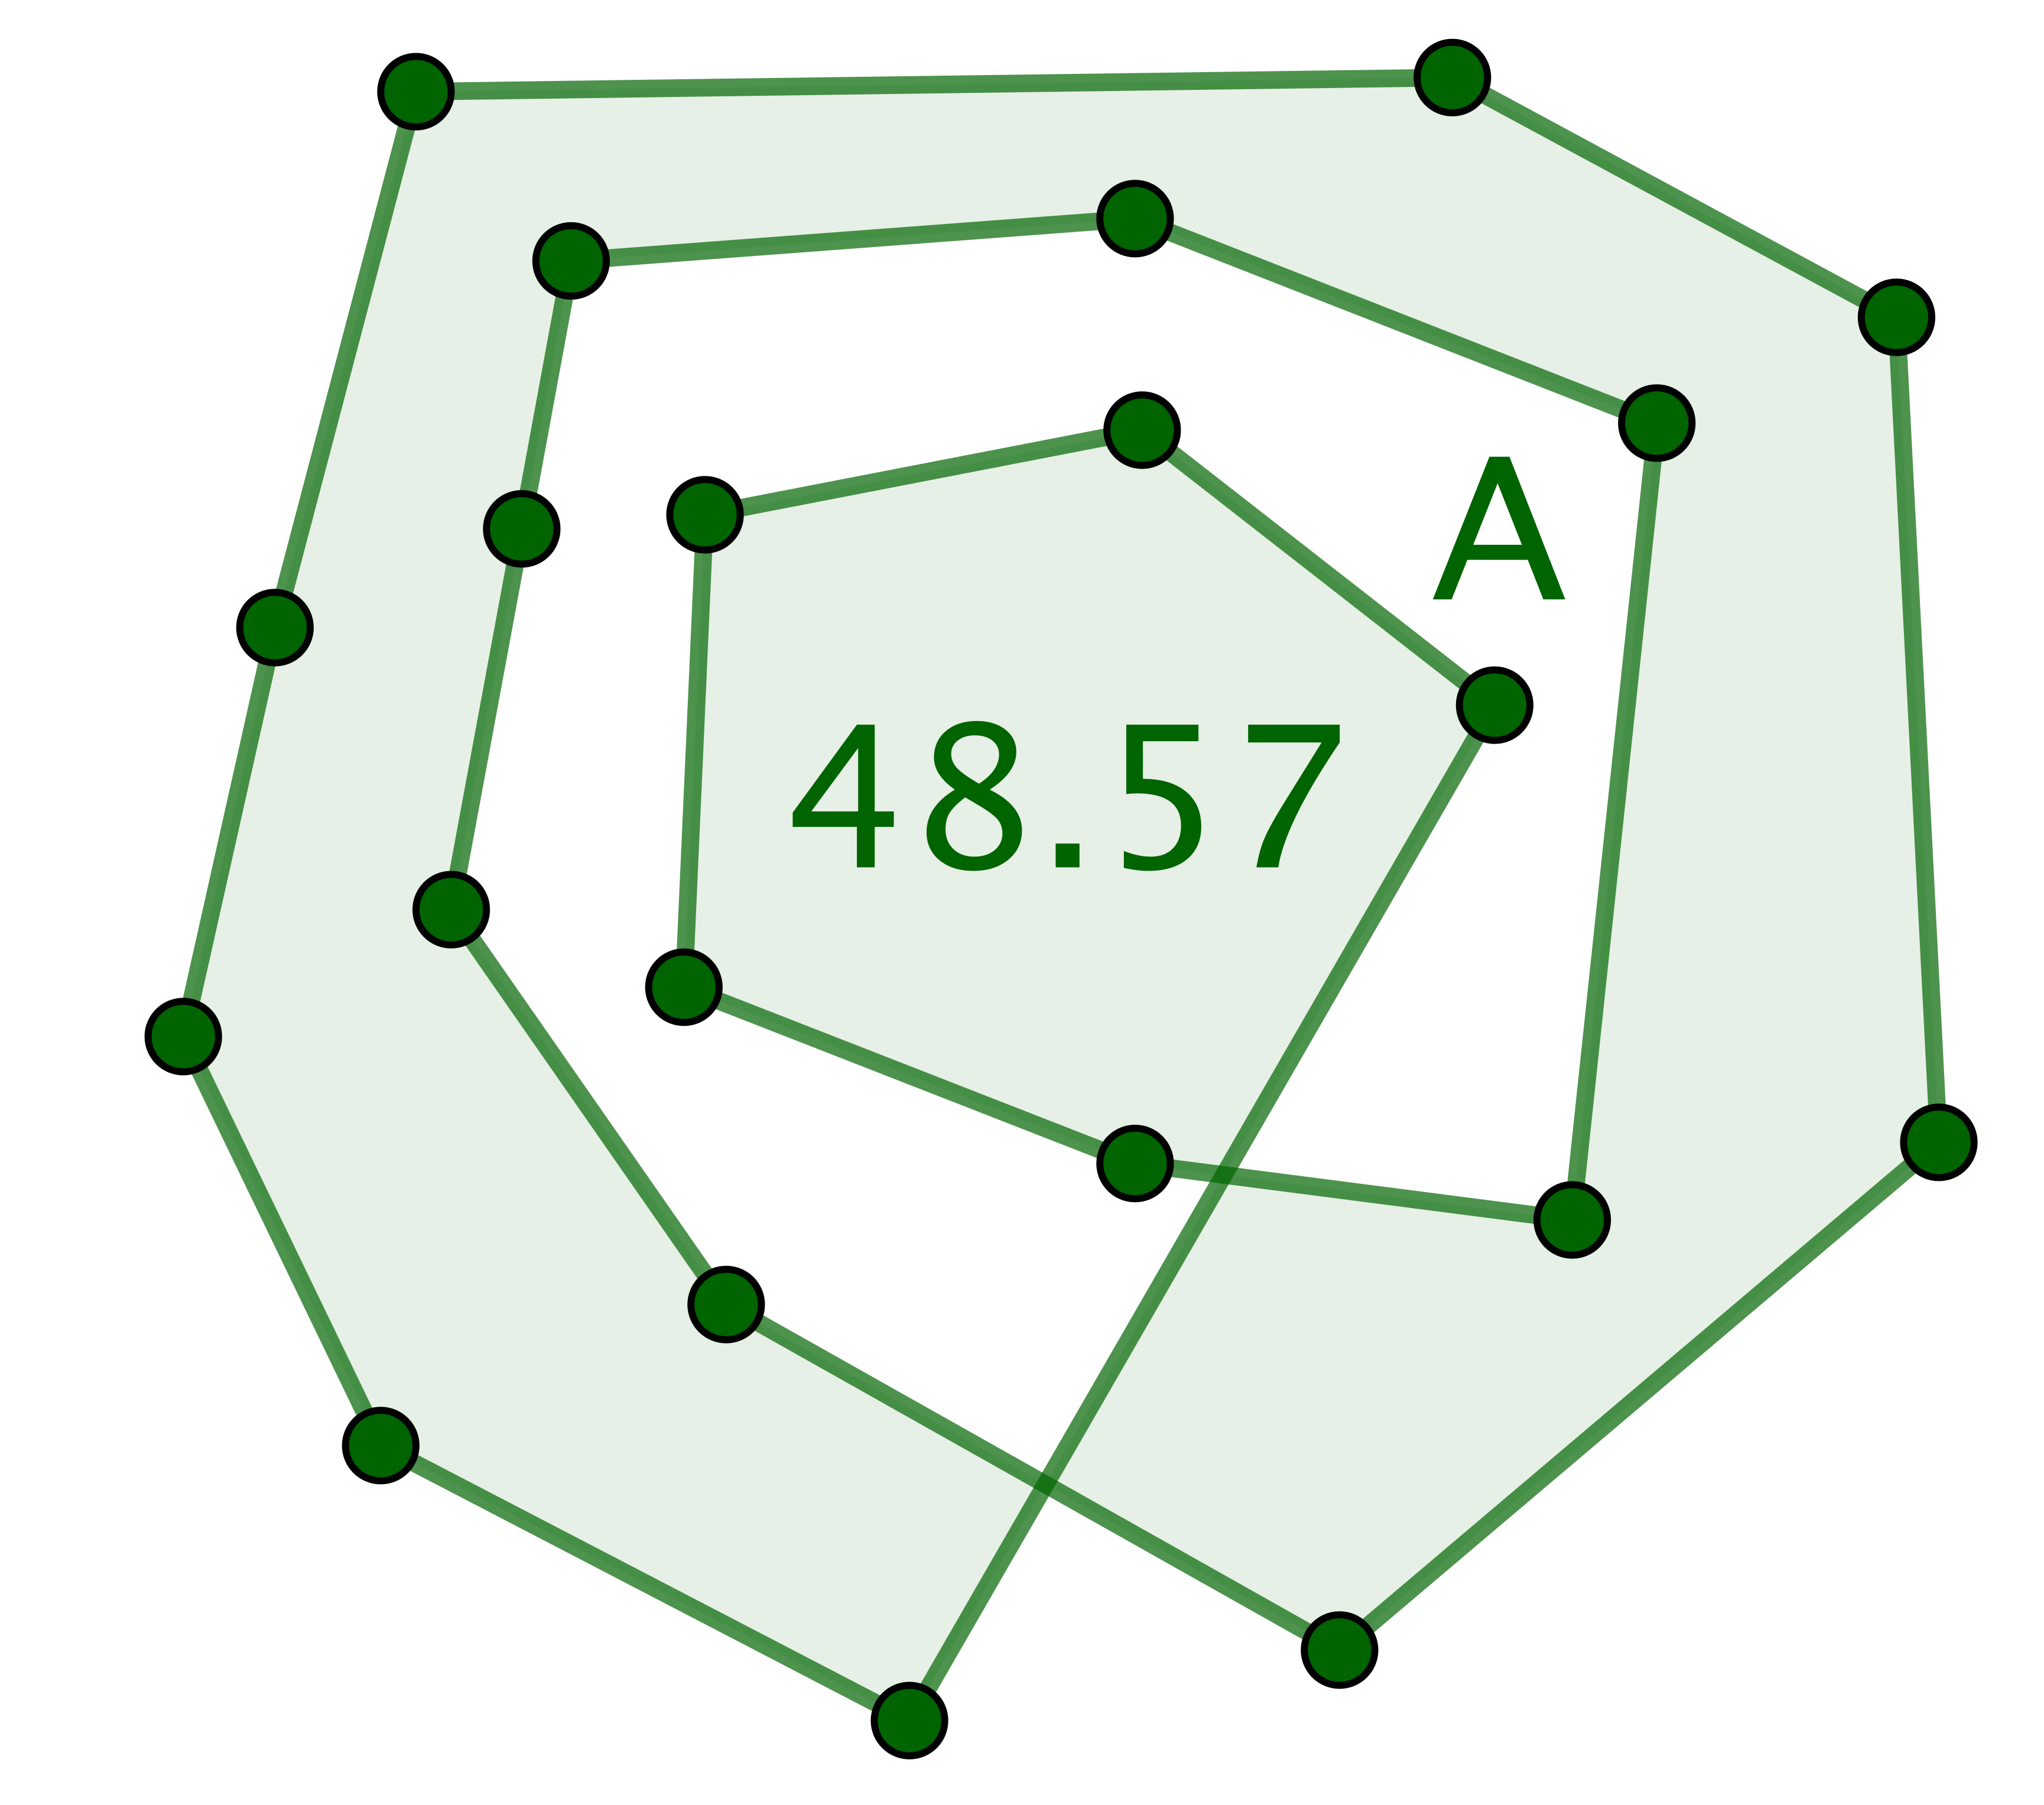
\includegraphics[scale=.3]{content/polygon/alg-area/alg-area-ncycle-not-opti-pb-1.png}

	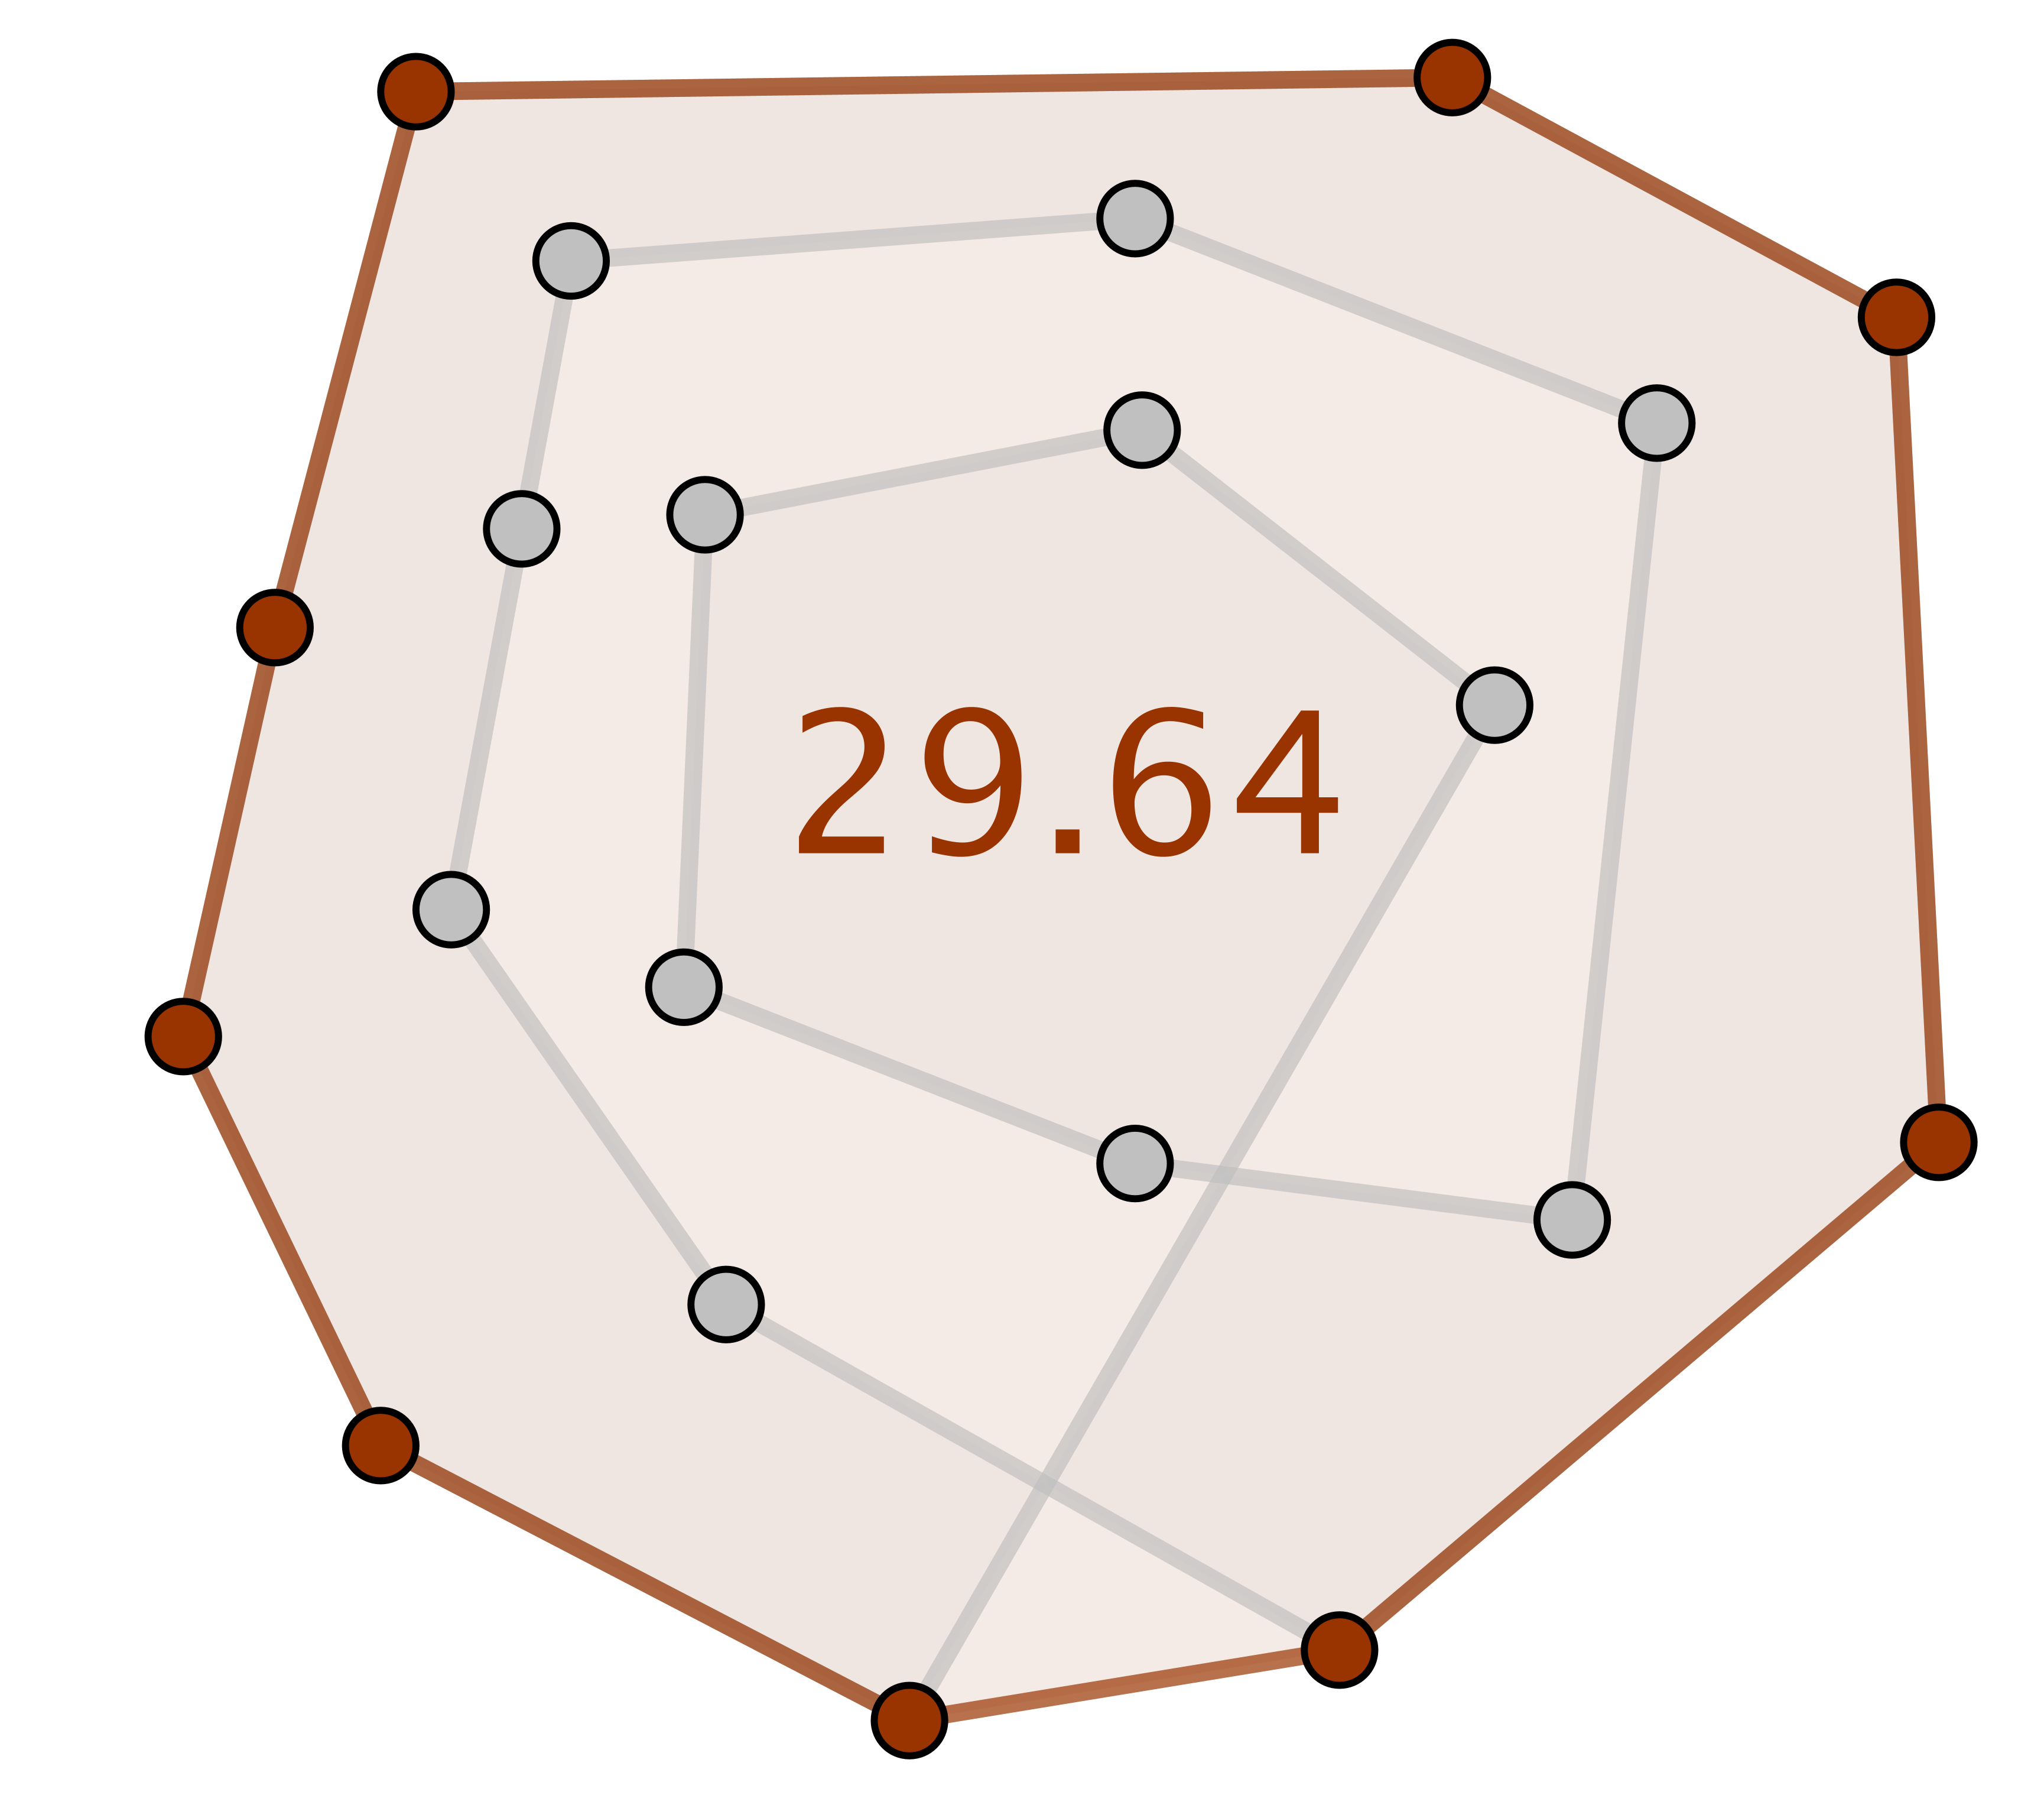
\includegraphics[scale=.3]{content/polygon/alg-area/alg-area-ncycle-not-opti-pb-2.png}
\end{multicols}


% ----------------------- %


Au commencement étaient les triangles... Il est connu que $ABC$ est d'aire $\frac12 \abs{ \det \big( \vect{AB} , \vect{AC} \big) }$ où $\frac12 \det \big( \vect{AB} , \vect{AC} \big)$ est appelé aire algébrique de $ABC$. Pour passer aux polygones, il \og suffit \fg\ d'utiliser des triangles comme dans l'exemple suivant.


\begin{multicols}{2}
	\small\itshape
    \begin{center}
		Calcul direct à la main.

		\smallskip

        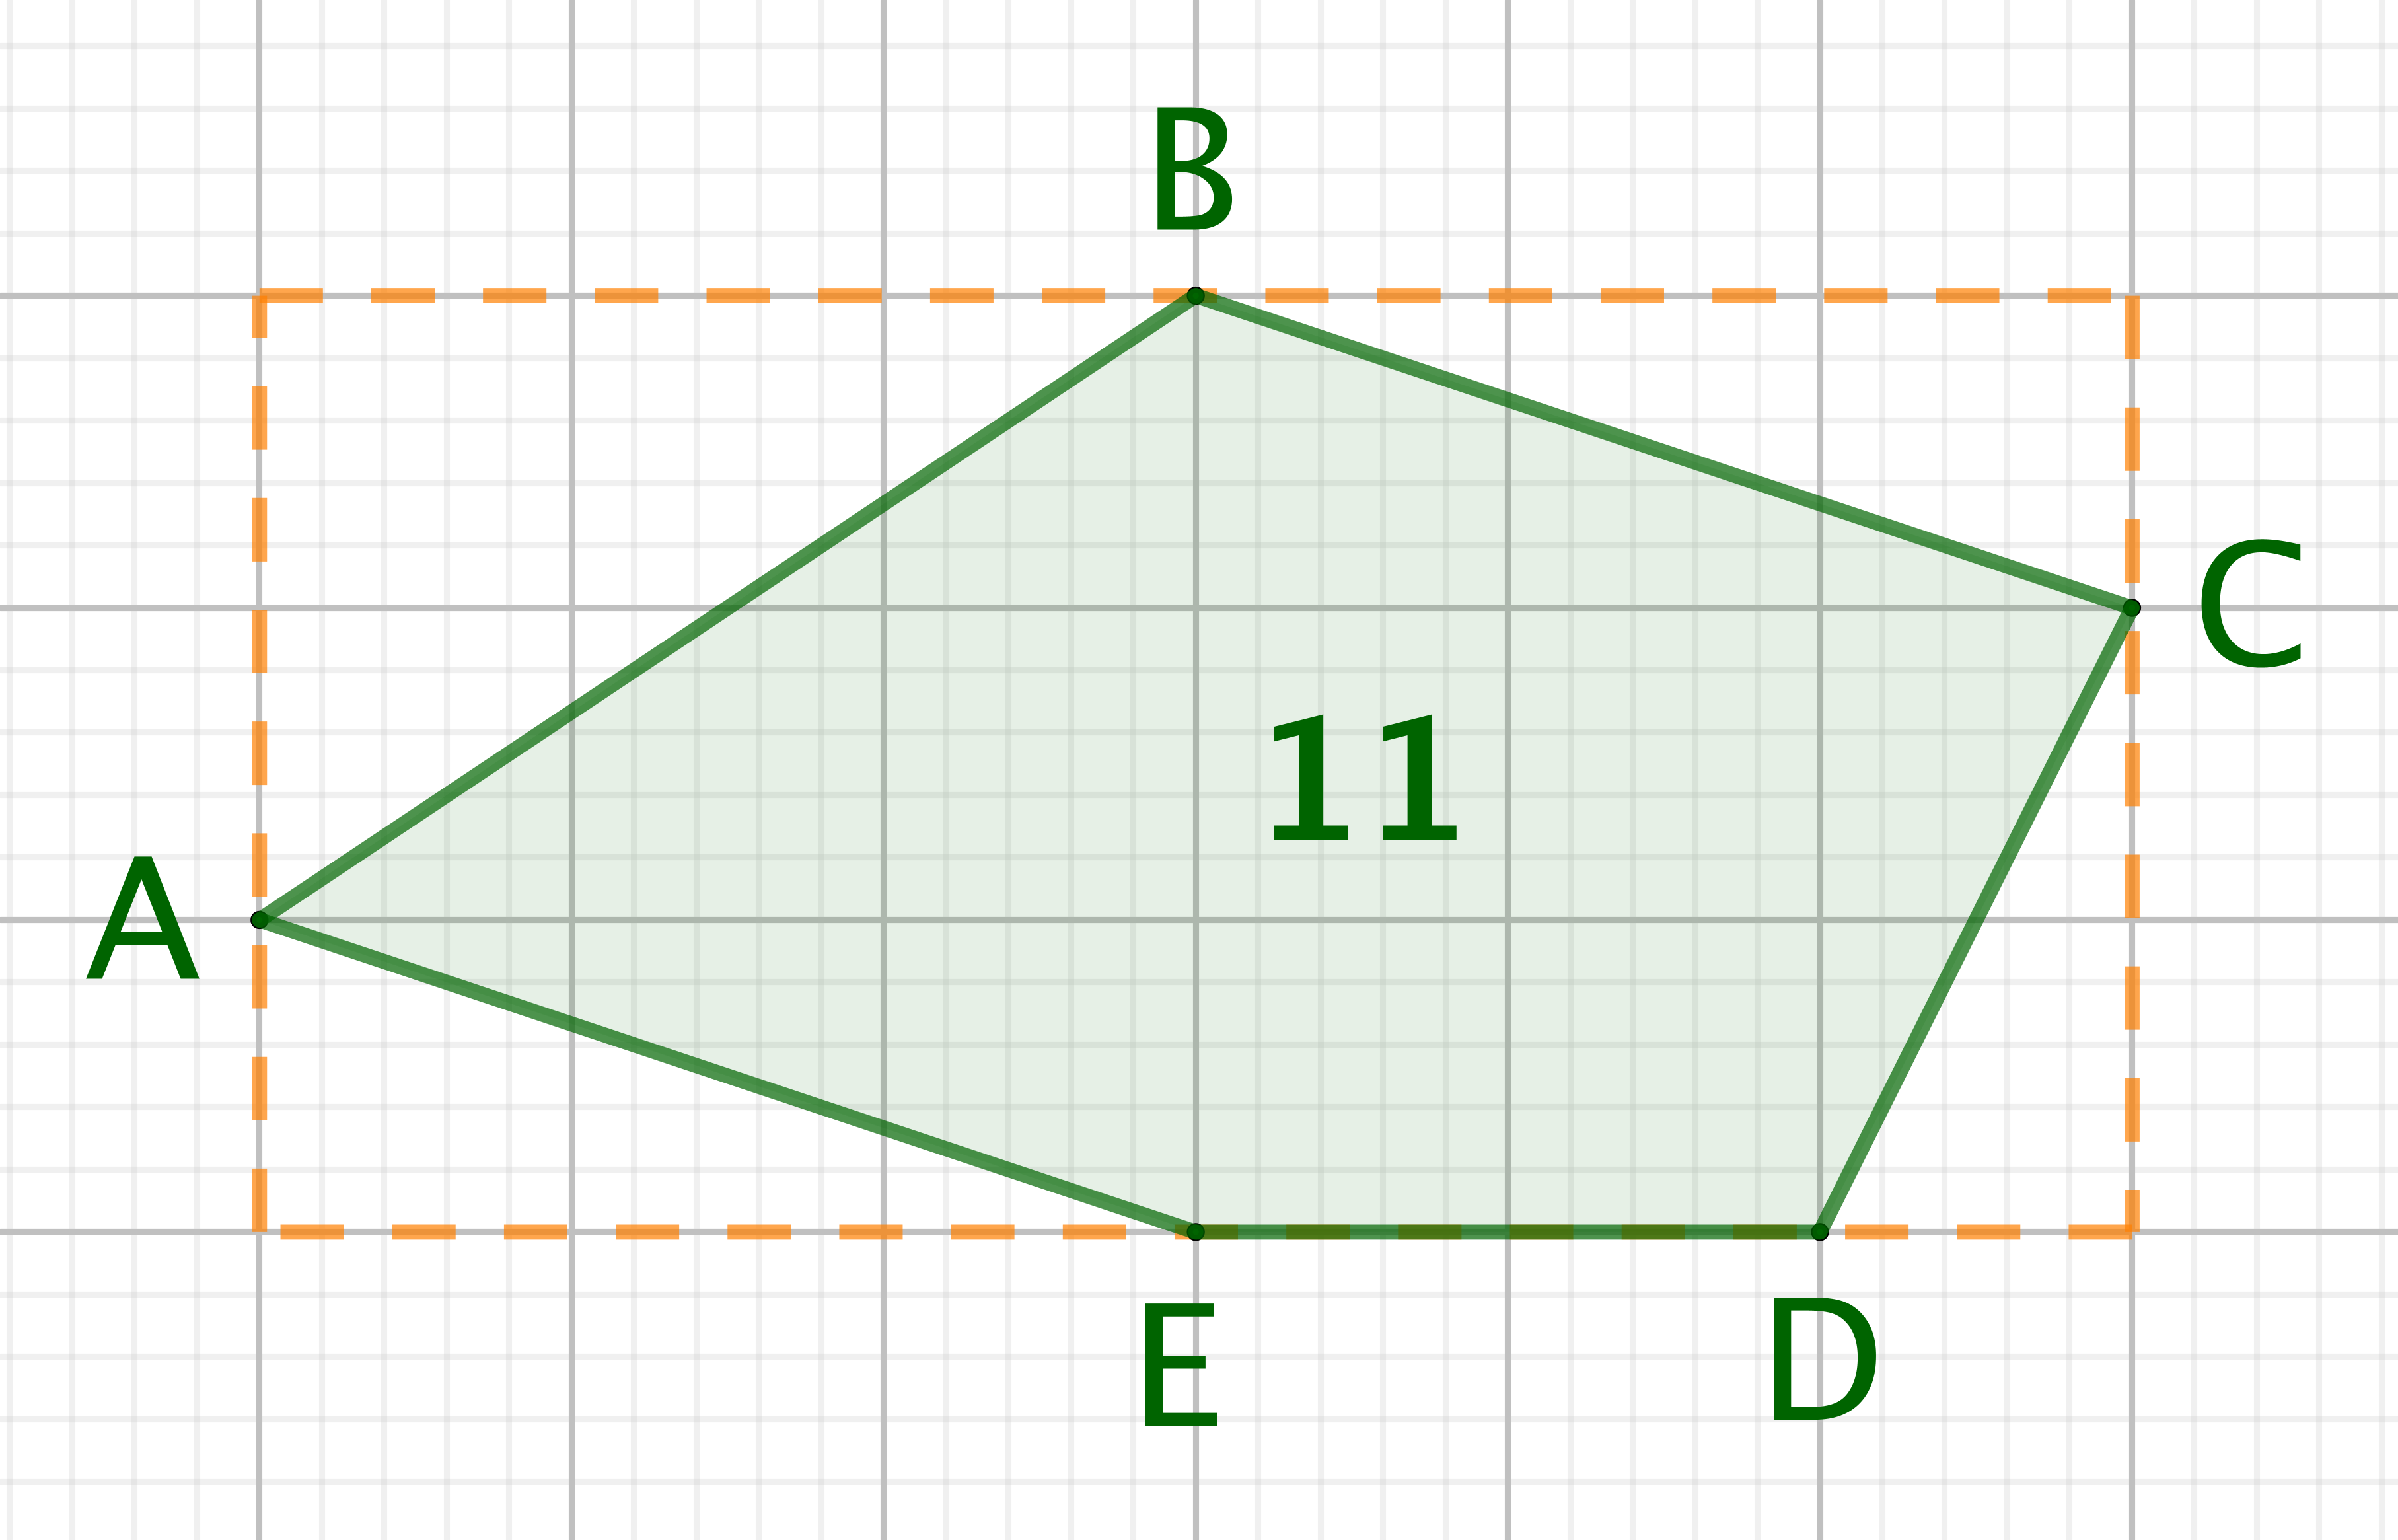
\includegraphics[scale=.35]{content/polygon/alg-area/convex-1.png}

       	\smallskip

		$11 = 3 \cdot 6 - \dfrac{3 \cdot 1 + 3 \cdot 2 + 3 \cdot 1 + 1 \cdot 2}{2} \vphantom{\dfrac{2^M}2}$
    \end{center}

	\columnbreak

    \begin{center}
		Via le déterminant.

		\smallskip

        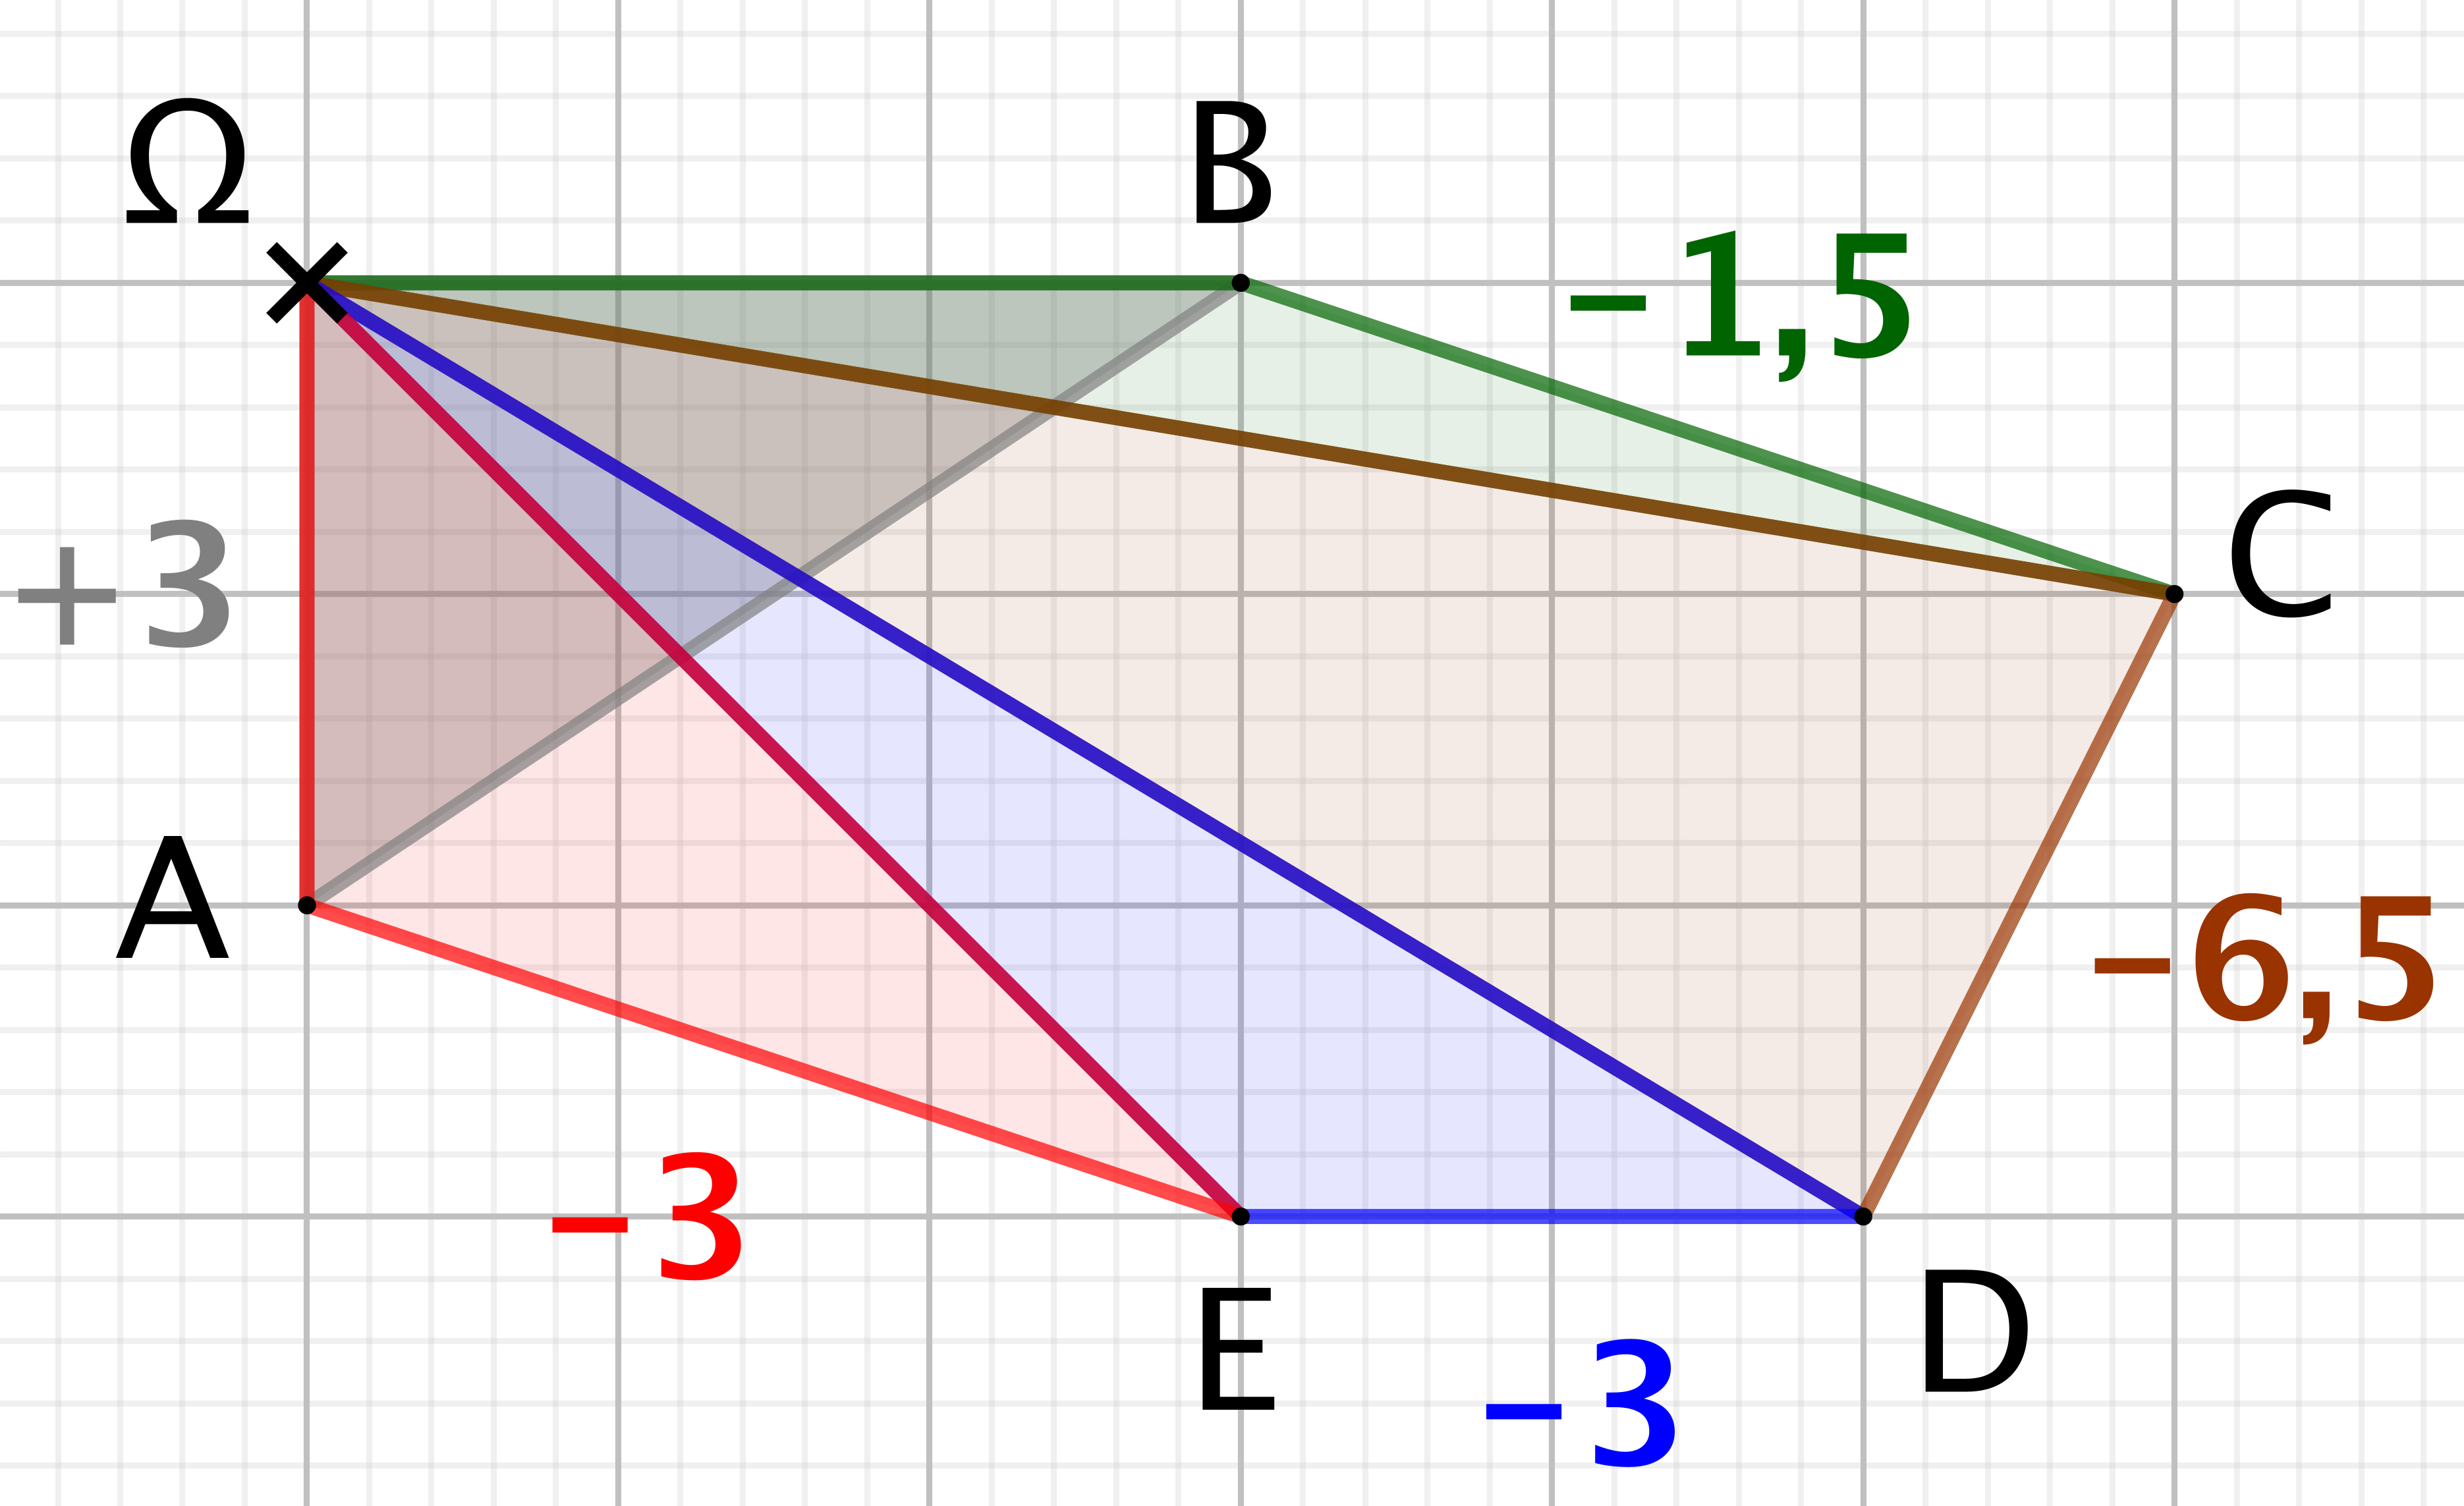
\includegraphics[scale=.35]{content/polygon/alg-area/convex-2.png}

       	\smallskip

		$- 11 = 3 - \num{1.5} - \num{6.5} - 3 - 3 \vphantom{\dfrac{2^M}2}$
    \end{center}
\end{multicols}


Dans le cas précédent, le résultat pourrait dépendre du point $\Omega$ employé, mais le fait suivant nous montre que non. Bonne nouvelle! Yapluka...


% ----------------------- %


\begin{fact} \label{sarea-pt-ct}
    Soit $\setproba{L} = A_1 A_2 \cdots A_n$ un \ncycle.
    La quantité
    $\mu_1^n (\Omega ;\setproba{L}) = \dsum_{i=1}^{n} \det \big( \vect{\Omega \primeit{A}_i} , \vect{\Omega \primeit{A}_{i+1}} \big)$ 
    est indépendante du point $\Omega$.
    Dans la suite, cette quantité indépendante de $\Omega$ sera notée $\mu_1^n (\setproba{L})$.
\end{fact}


\begin{proof}
    Soit $M$ un autre point du plan.

    \begin{stepcalc}[style=ar*]
        \mu_1^n (\Omega ;\setproba{L})
    \explnext{}
        \dsum_{i=1}^{n} \det \big( \vect{\Omega \primeit{A}_i} , \vect{\Omega \primeit{A}_{i+1}} \big)
    \explnext{}
        \dsum_{i=1}^{n} \det \big( \vect{\Omega M} + \vect{M \primeit{A}_i} , \vect{\Omega M} + \vect{M \primeit{A}_{i+1}} \big)
    \explnext{}
        \dsum_{i=1}^{n} \Big[
            \det \big( \vect{\Omega M} , \vect{\Omega M} \big)
            +
            \det \big( \vect{\Omega M} , \vect{M \primeit{A}_{i+1}} \big)
            +
            \det \big( \vect{M \primeit{A}_i} , \vect{\Omega M} \big)
            +
            \det \big( \vect{M \primeit{A}_i} , \vect{M \primeit{A}_{i+1}} \big)
        \Big]
    \explnext{}
        \dsum_{i=1}^{n} \det \big( \vect{\Omega M} , \vect{M \primeit{A}_{i+1}} \big)
        +
        \dsum_{i=1}^{n} \det \big( \vect{M \primeit{A}_i} , \vect{\Omega M} \big)
        +
        \mu_1^n (M ; \setproba{L})
    \explnext{}
        \dsum_{i=2}^{n+1} \det \big( \vect{\Omega M} , \vect{M \primeit{A}_{i}} \big)
        -
        \dsum_{i=1}^{n} \det \big( \vect{\Omega M} , \vect{M \primeit{A}_i} \big)
        +
        \mu_1^n (M ; \setproba{L})
    \explnext*{$\primeit{A}_{n+1} = \primeit{A}_1$}{}
        \mu_1^n (M ; \setproba{L})
    \end{stepcalc}

    \null\vspace{-3.5ex}
\end{proof}


% ----------------------- %


\begin{fact} \label{nline-shift-inva}
    Soient $\setproba{L} = A_1 A_2 \cdots A_n$ un \ncycle,
    et
    l'un de ses\ \og \emph{permutés} \fg\ $\setproba{L}_k = B_1 B_2 \cdots B_n$ défini par $B_i = \primeit{A}_{i+k}$ pour $k \in \ZZ$,
    %
    Nous avons
    $\mu_1^n (\setproba{L}) = \mu_1^n (\setproba{L}_k)$.
    Cette quantité commune sera notée $\mu (\setproba{L})$.
\end{fact}


\begin{proof}
    Il suffit de s'adonner à un petit jeu sur les indices de sommation.
\end{proof}


% ----------------------- %


\begin{fact} \label{nline-rota-opp}
    Soient
    $\setproba{L} = A_1 A_2 \cdots A_n$ un \ncycle,
    et
    son \ncycle\ \og \emph{opposé} \fg\ $\cycleop{L} = B_1 B_2 \cdots B_n$ où $B_i =  A_{n + 1 - i}$.
    %
    Nous avons
    $\mu(\cycleop{L}) = - \mu(\setproba{L})$.
\end{fact}


\begin{proof}
    Soit $\Omega$ un point quelconque du plan.

    \begin{stepcalc}[style=ar*]
        \mu(\cycleop{L})
    \explnext{}
        \dsum_{i=1}^{n} \det \big( \vect{\Omega B^{\,\prime}_i} , \vect{\Omega B^{\,\prime}_{i+1}} \big)
    \explnext*{$B^{\,\prime}_i =  \primeit{A}_{n + 1 - i}$ et $j = n - i$}{}
%        \dsum_{i=1}^{n} \det \big( \vect{\Omega \primeit{A}_{n + 1 - i}} , \vect{\Omega \primeit{A}_{n - i}} \big)
%    \explnext{}
        \dsum_{j=0}^{n-1} \det \big( \vect{\Omega \primeit{A}_{j + 1}} , \vect{\Omega \primeit{A}_j} \big)
    \explnext*{$\primeit{A}_0 = \primeit{A}_n$ et $\primeit{A}_1 = \primeit{A}_{n+1}$}{}
%        \dsum_{j=1}^{n} \det \big( \vect{\Omega \primeit{A}_{j + 1}} , \vect{\Omega \primeit{A}_j} \big)
%    \explnext{}
        - \dsum_{j=1}^{n} \det \big( \vect{\Omega \primeit{A}_j} , \vect{\Omega \primeit{A}_{j + 1}} \big)
    \explnext{}
        - \mu(\setproba{L})
    \end{stepcalc}

    \null\vspace{-3.5ex}
\end{proof}


% ----------------------- %


\begin{fact} \label{sarea-ncycle}
    Soit
    $\setproba{L} = A_1 A_2 \cdots A_n$ un \ncycle.
    La quantité $\sarea{\setproba{L}} = \frac12 \mu(\setproba{L})$ ne dépend que du sens de parcours de $\setproba{L}$, mais pas de l'origine.%
    \footnote{
        Le lecteur pardonnera les abus de langage utilisés.
    }
    Elle sera appelée \og \emph{aire algébrique} \fg\ de $\setproba{L}$.
\end{fact}


\begin{proof}
    C'est une conséquence directe des faits \ref{nline-shift-inva} et \ref{nline-rota-opp}.
\end{proof}


% ----------------------- %


Considérons, maintenant, un \ngone\ convexe $\setproba{P} = A_1 A_2 \cdots A_n$ où les sommets sont parcourus dans le sens anti-horaire.
En choisissant l'isobarycentre $G$ des points $A_1$, $A_2$, ..., $A_n$ pour calculer $\sarea{\setproba{P}}$, nous obtenons $\area{\setproba{P}} = \sarea{\setproba{P}}$:
en effet,
avec ce choix, tous les déterminants $\det \big( \vect{G \primeit{A}_i} , \vect{G \primeit{A}_{i+1}} \big)$ sont positifs.
Dans le cas non-convexe, les choses se compliquent a priori, car nous ne maîtrisons plus les signes des déterminants. Heureusement, nous avons le résultat essentiel suivant.


\begin{fact} \label{route-direction}
    Soit un \ngone\ $\setproba{P} = A_1 A_2 \cdots A_n$ tel que $A_1$, $A_2$, ..., $A_n$ soient parcourus dans le sens trigonométrique, ou anti-horaire.
    Un tel \ngone\ sera dit \focus{positif}.%
    \footnote{
    	De façon cachée, nous utilisons le célèbre théorème de Jordan, dans sa forme polygonale.
    }
    Sous cette hypothèse, nous avons 
    $\mu(\setproba{P}) \geq 0$,
    \emph{i.e.}
    $\sarea{\setproba{P}} \geq 0$.
\end{fact}


\begin{proof}
	Le théorème de triangulation affirme que tout \ngone\ est triangulable comme dans l'exemple suivant: ceci laisse envisager une démonstration par récurrence en retirant l'un des triangles ayant deux côtés correspondant à deux côtés consécutifs du \ngone\ (pour peu qu'un tel triangle existe toujours).


    \begin{multicols}{3}
        \small\itshape
        \begin{center}
            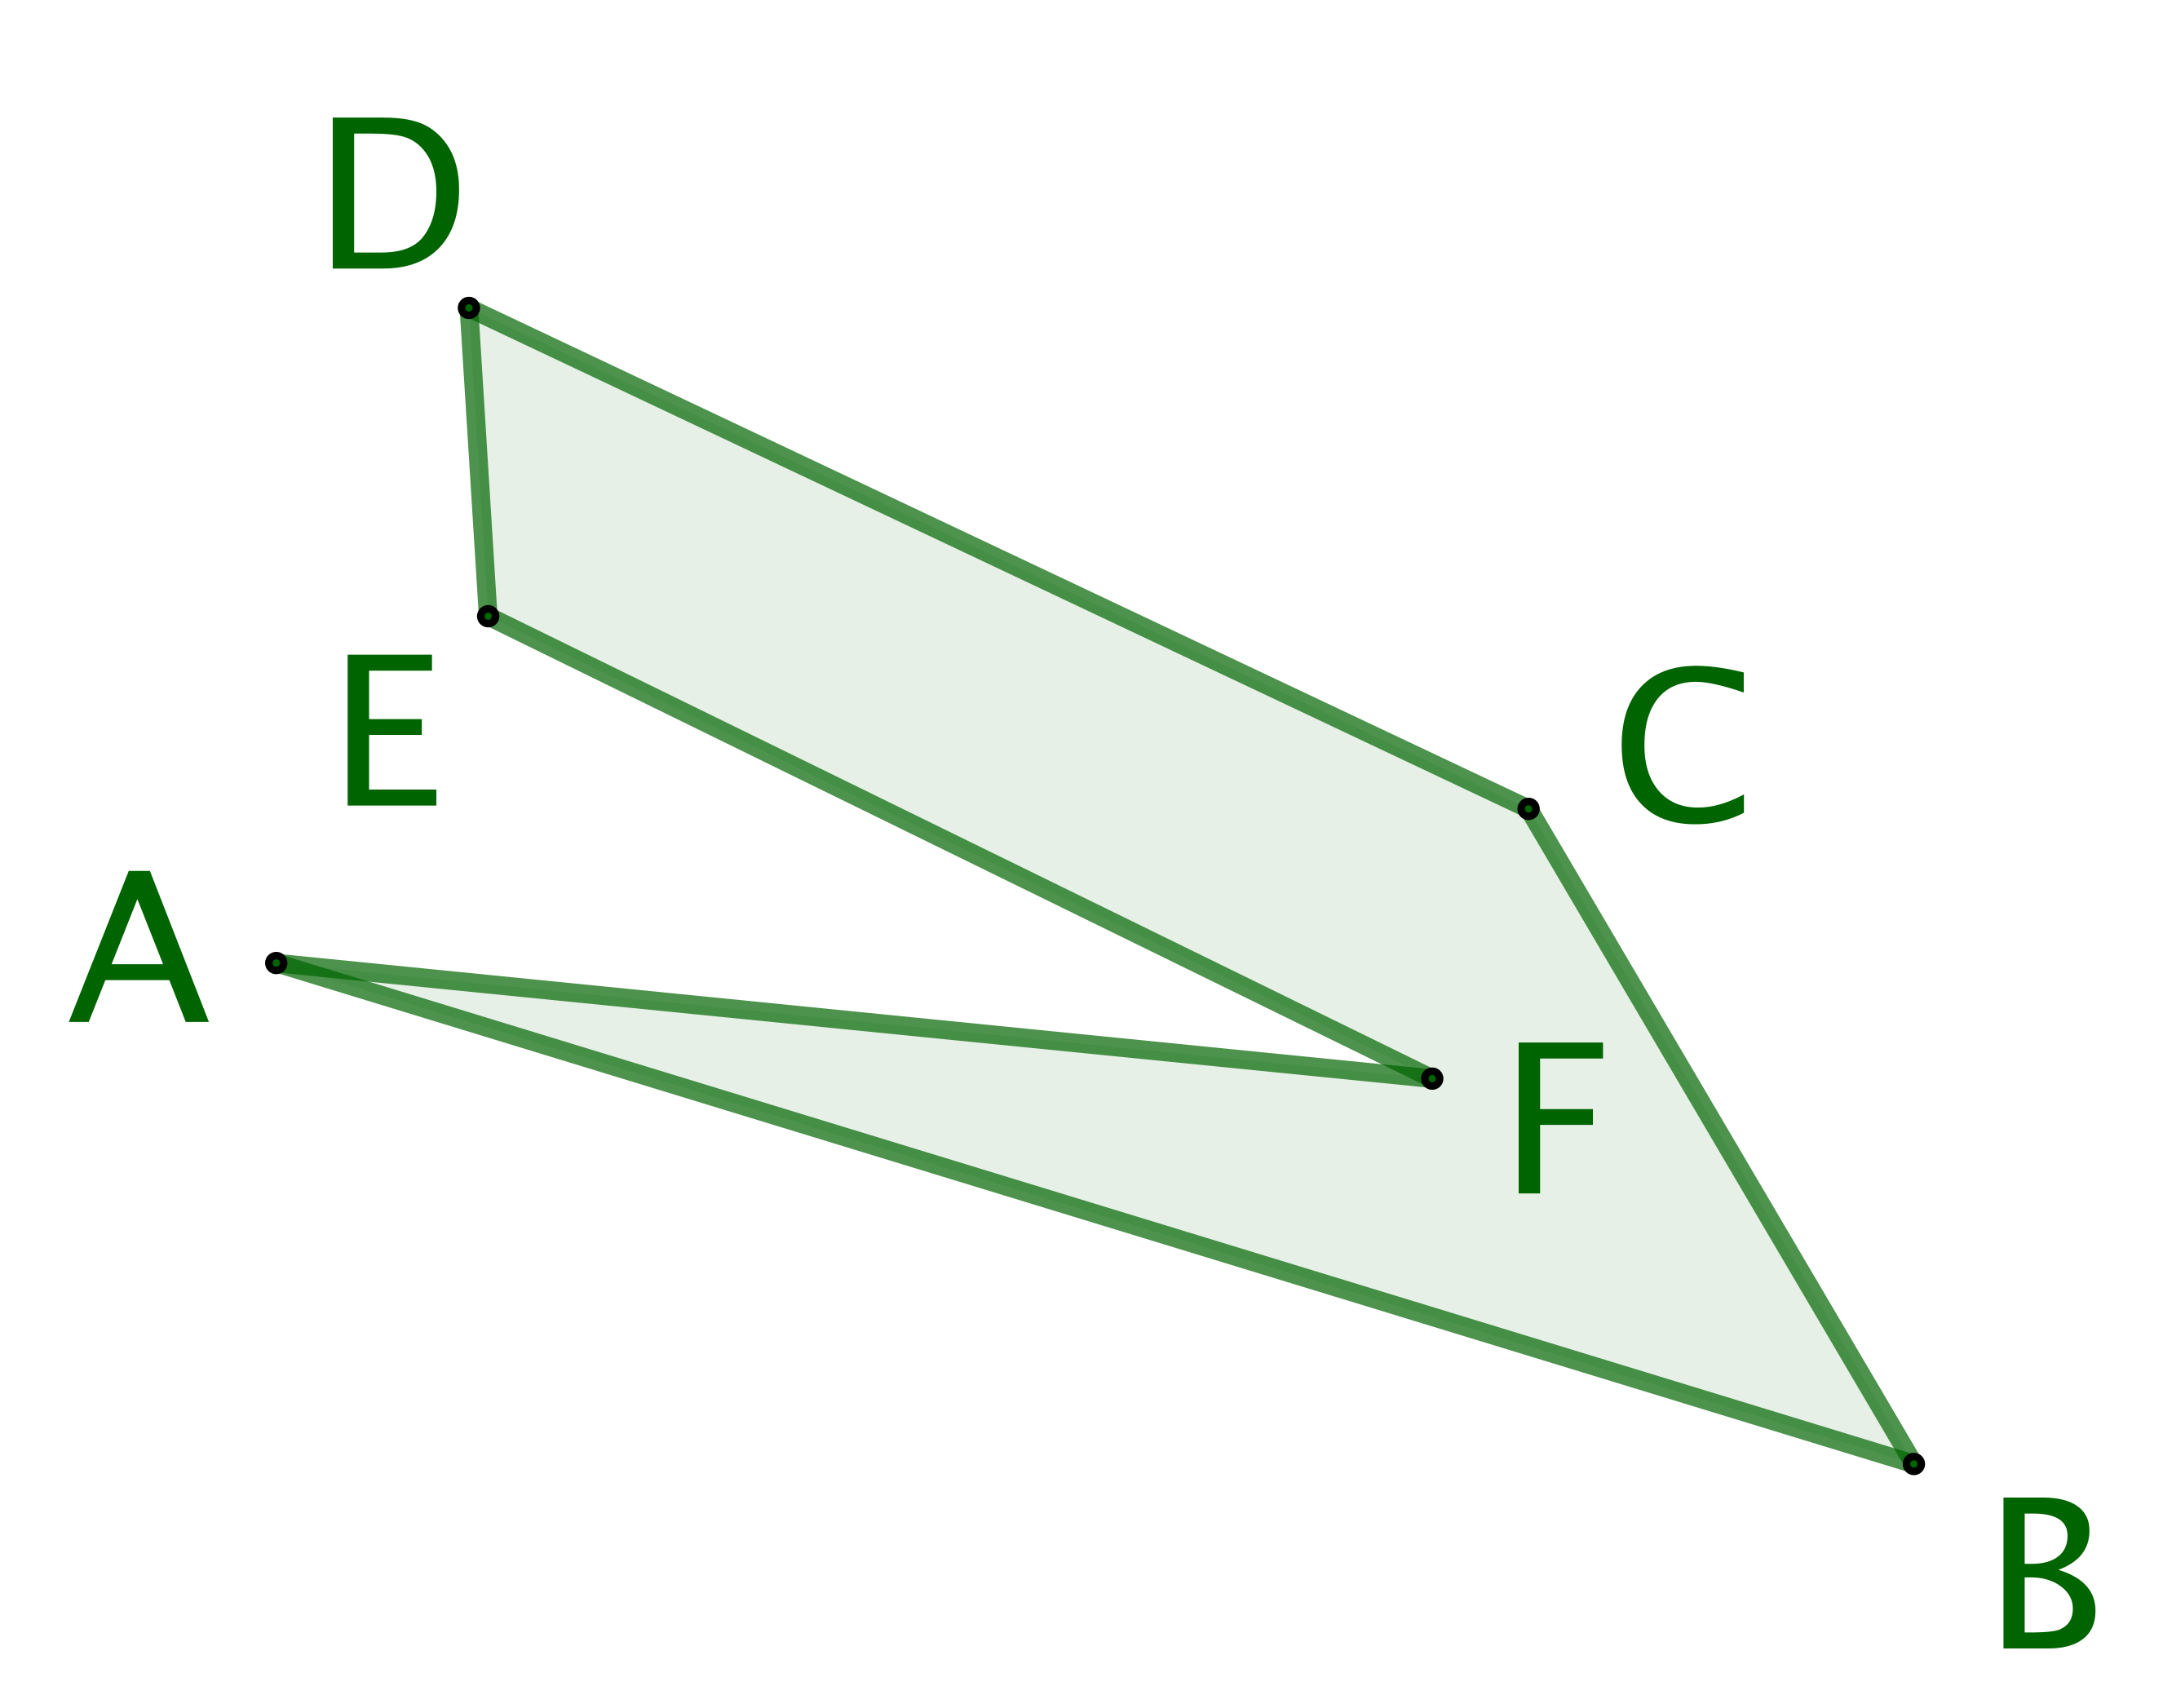
\includegraphics[scale=.4]{content/polygon/alg-area/triangulation-1.png}

            \smallskip
            Un \ngone\ \og nu \fg.
        \end{center}


        \begin{center}
            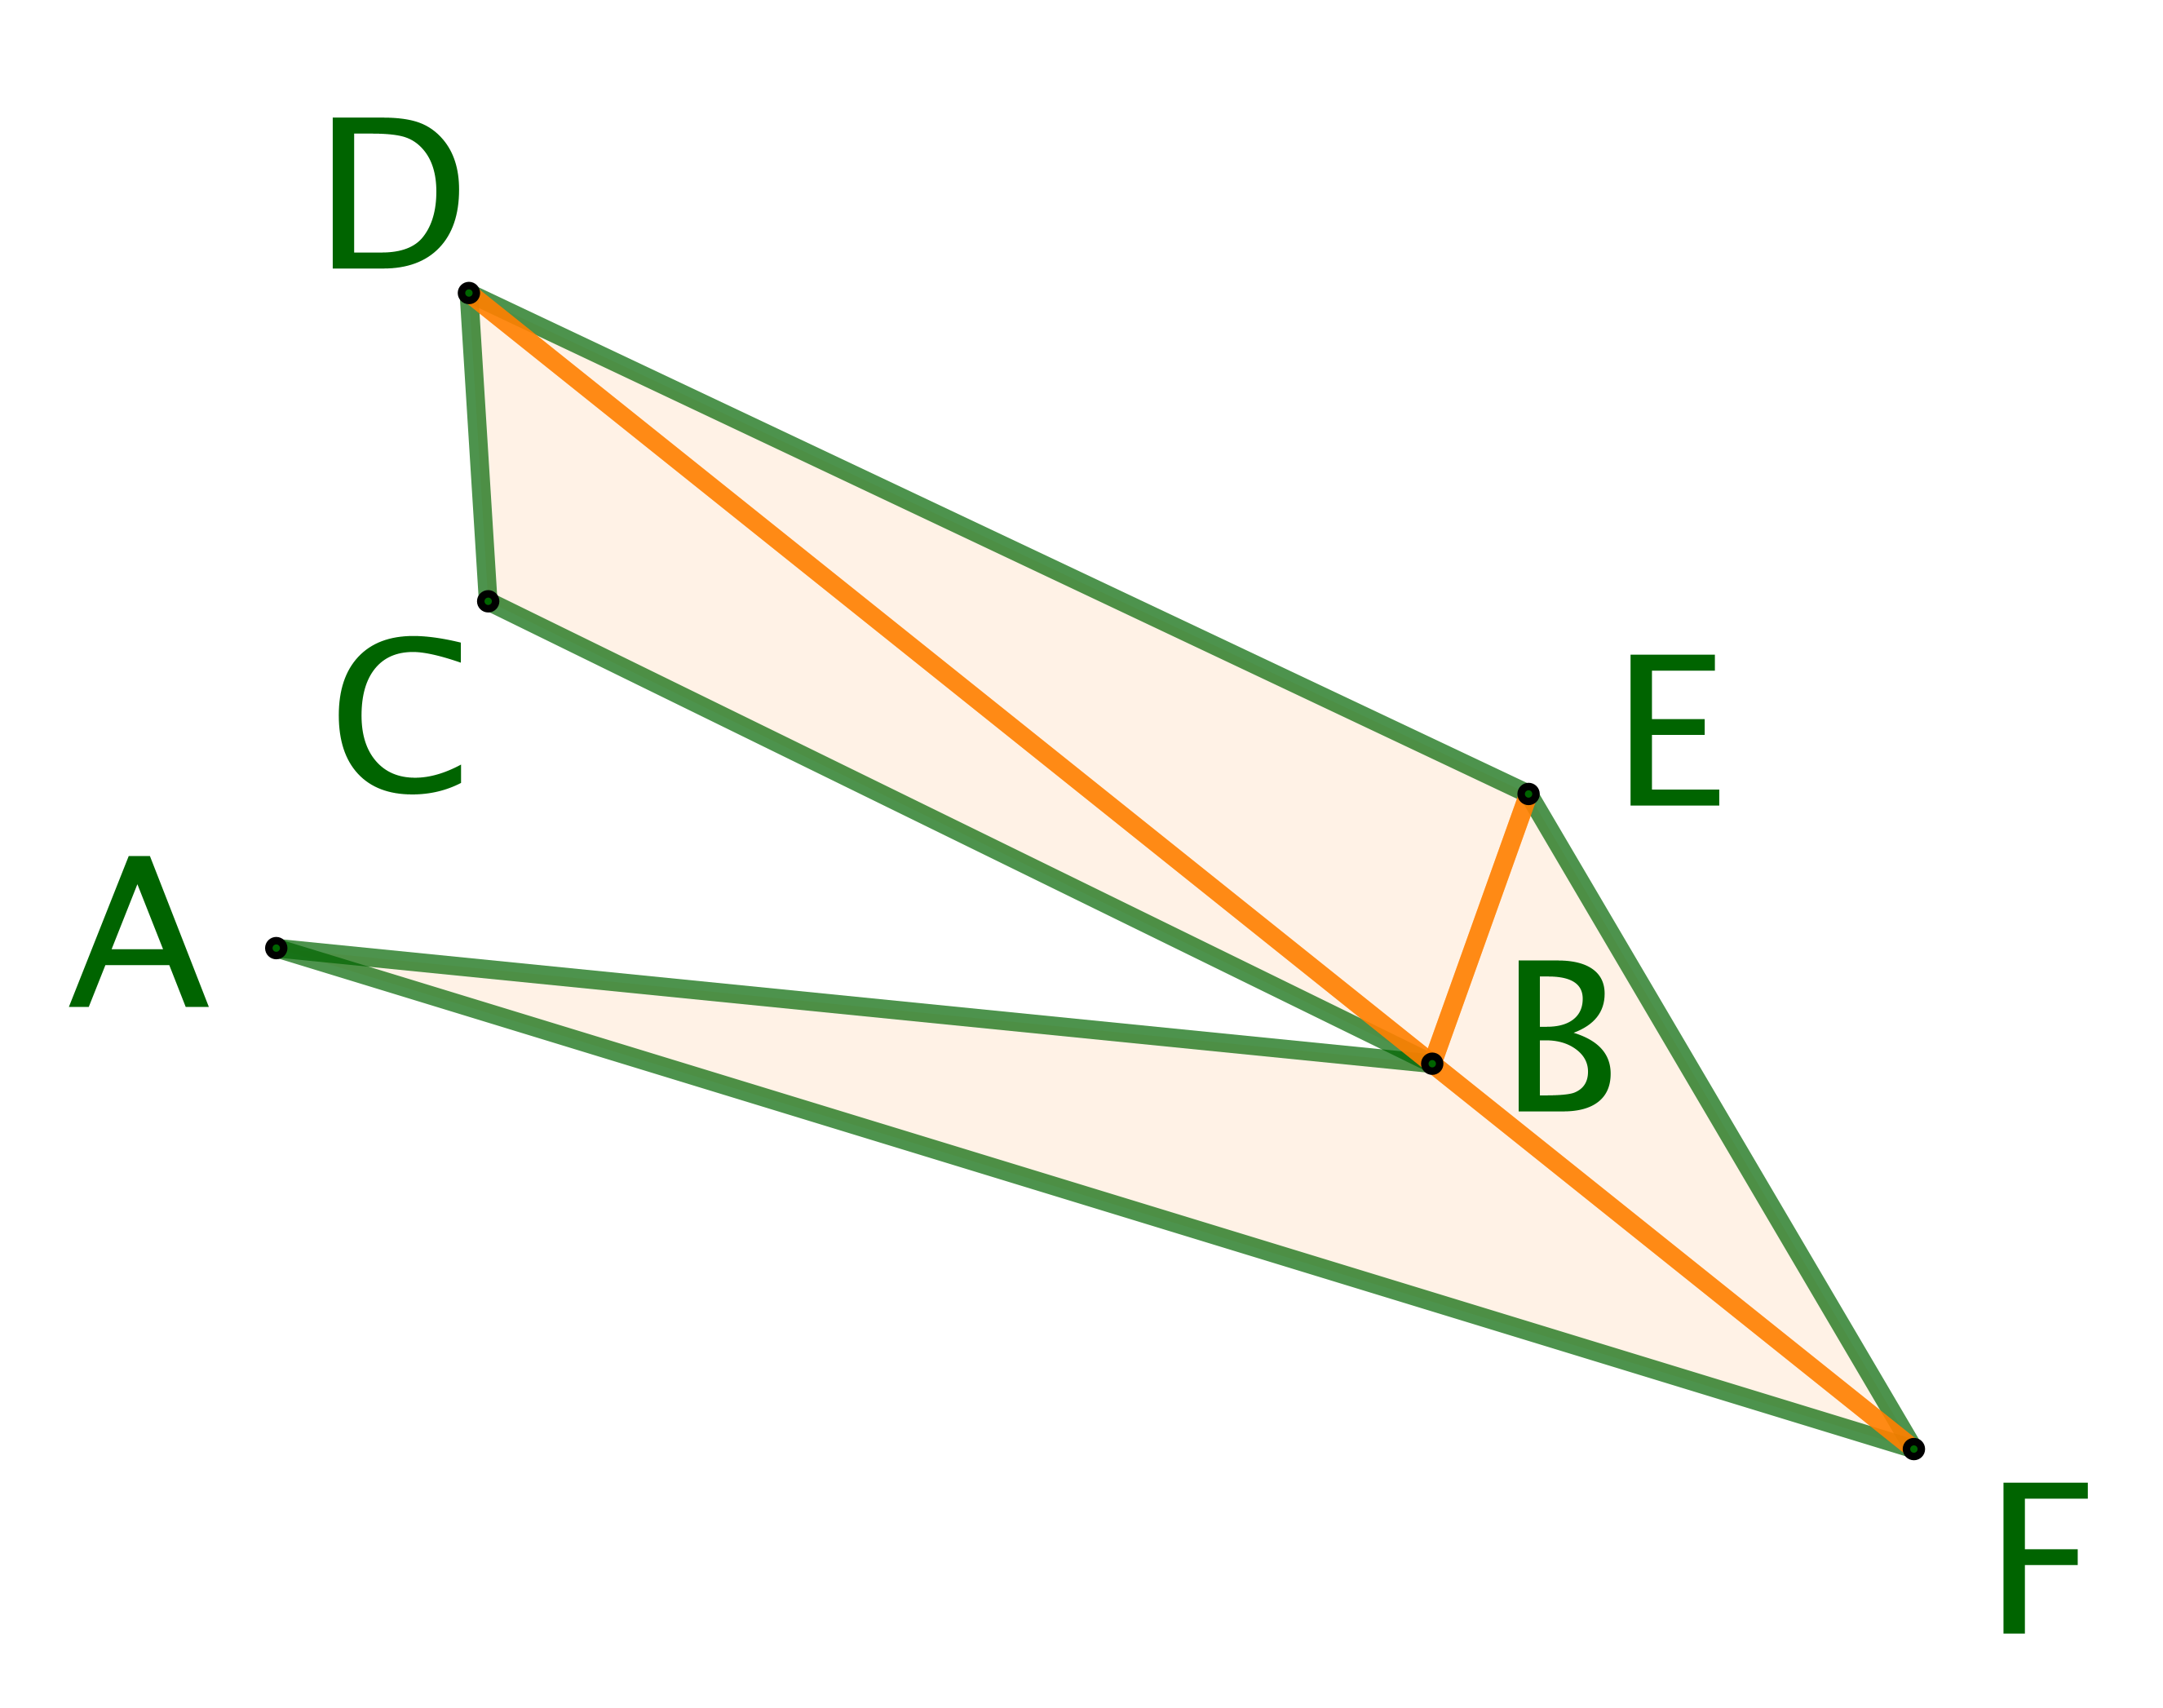
\includegraphics[scale=.4]{content/polygon/alg-area/triangulation-2.png}

            \smallskip
            Le \ngone\ triangulé.
        \end{center}


        \begin{center}
            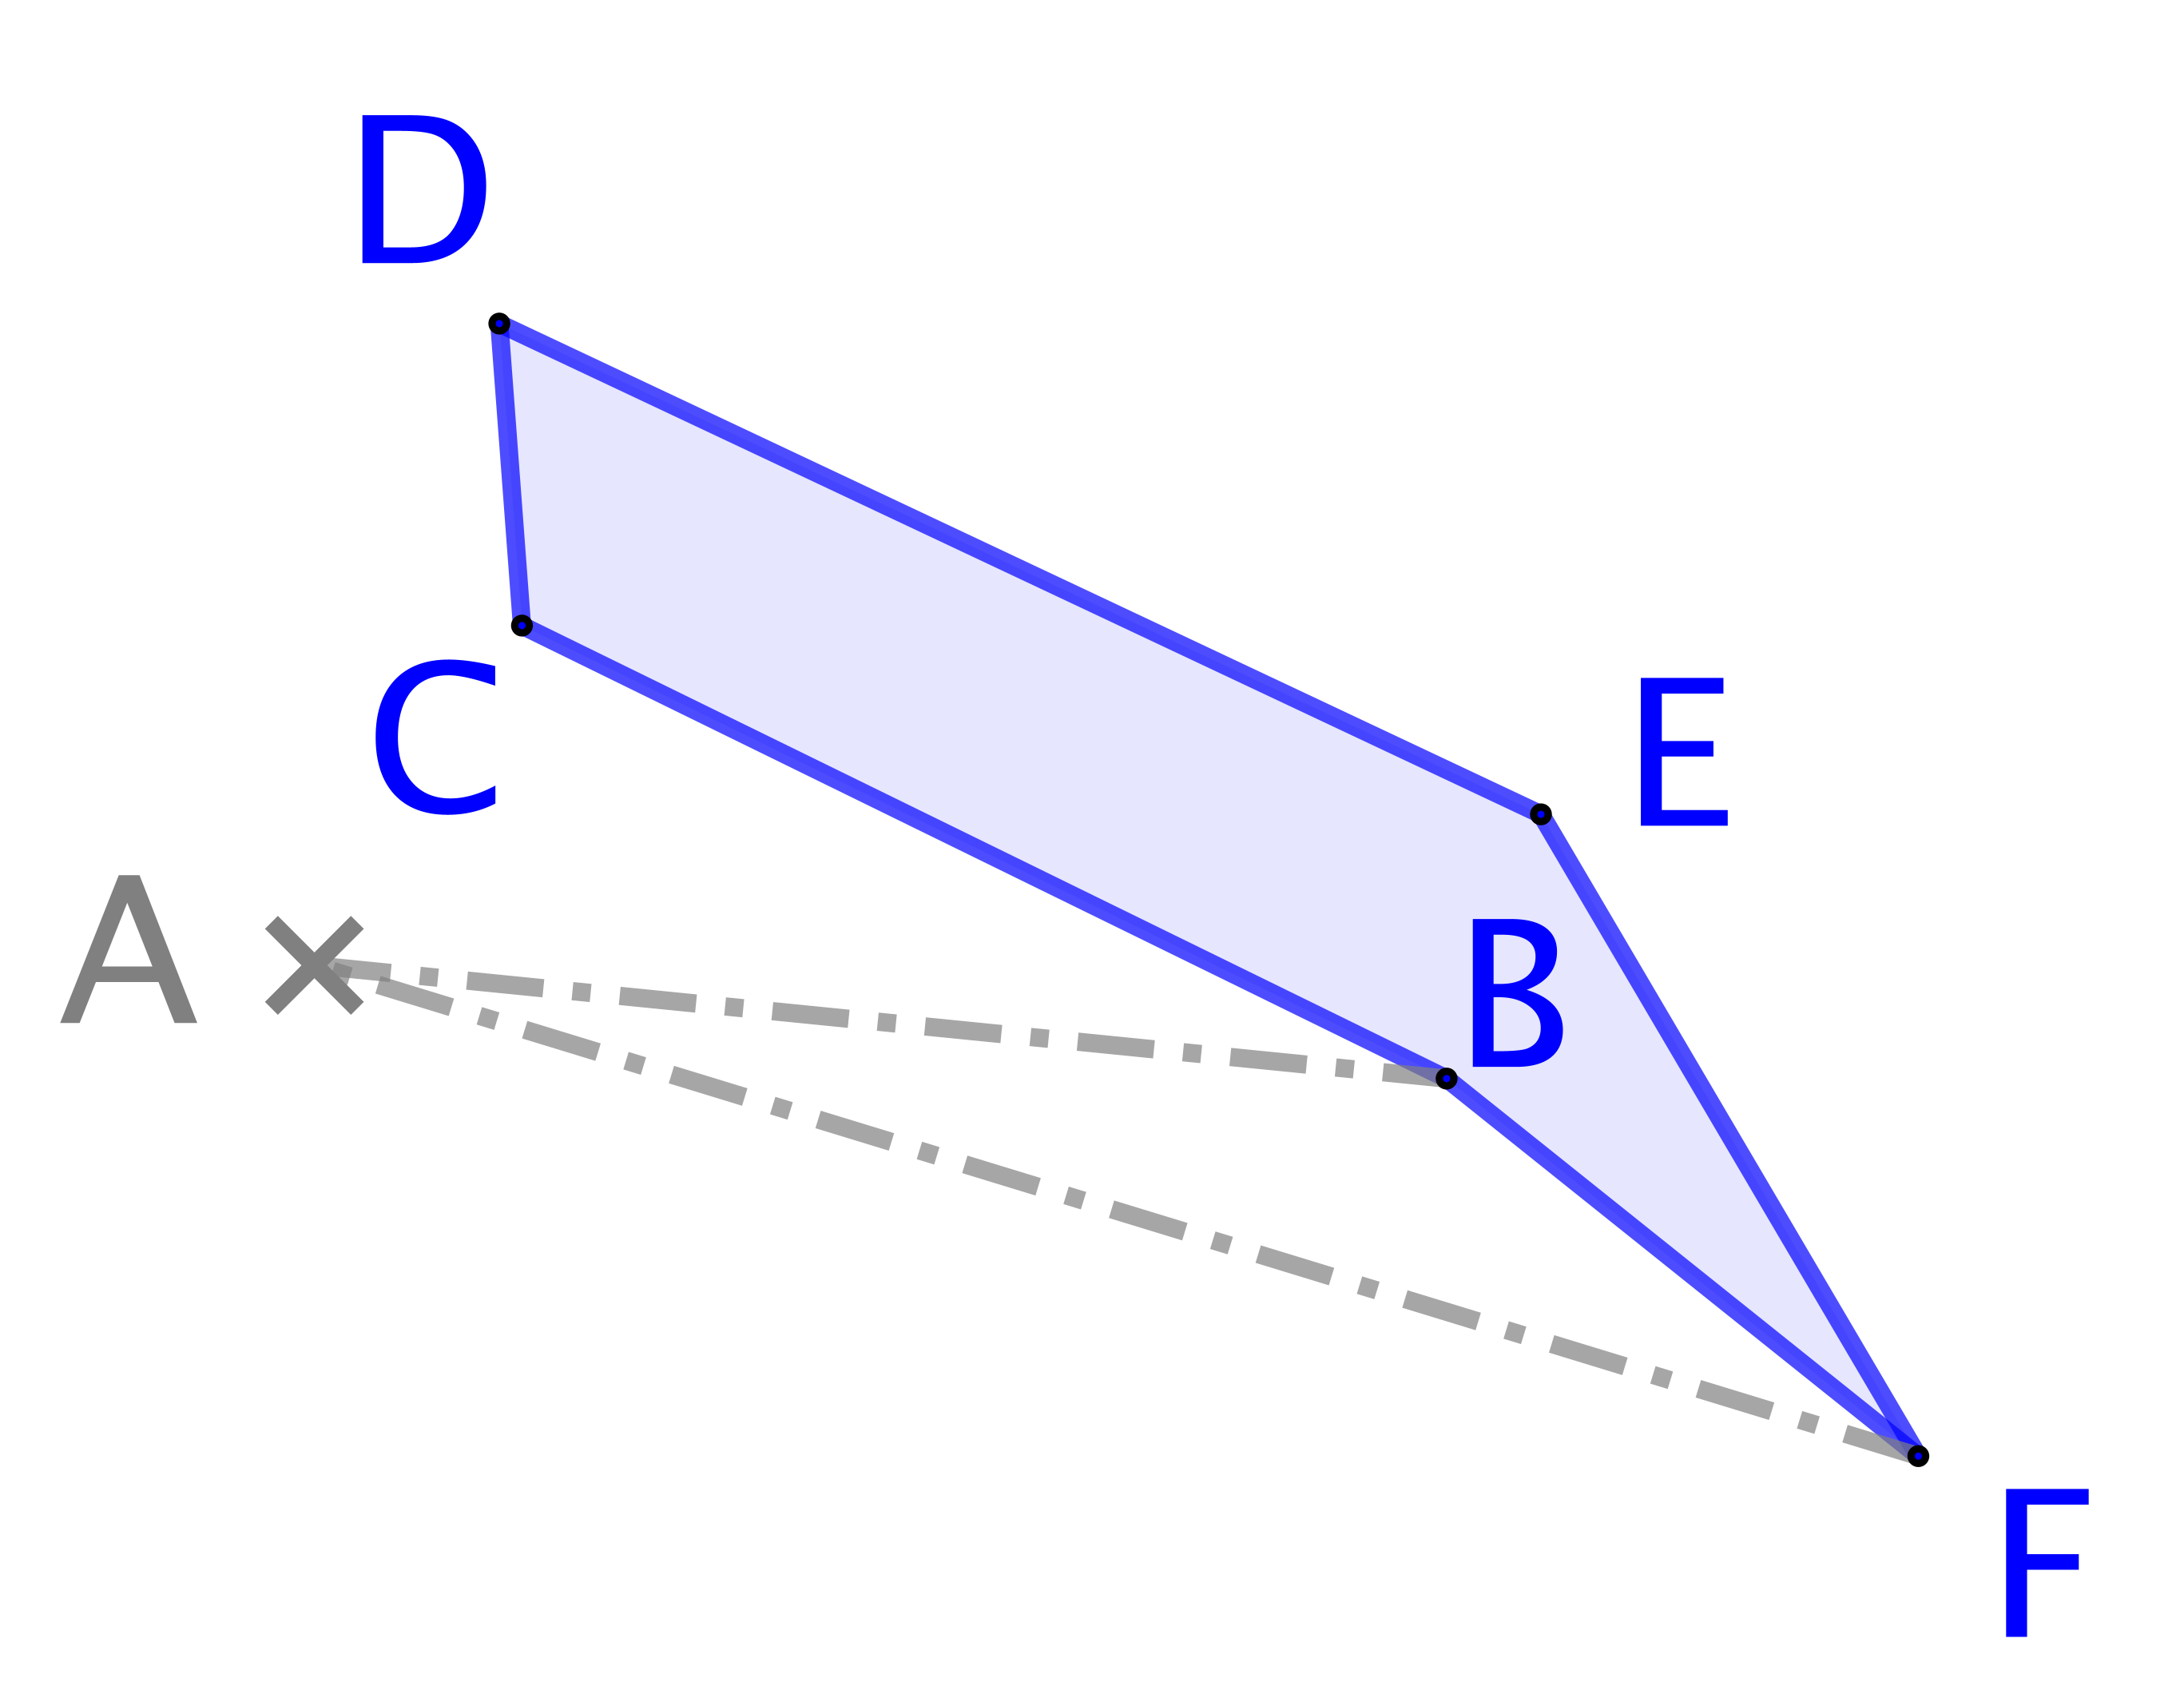
\includegraphics[scale=.4]{content/polygon/alg-area/triangulation-3.png}

            \smallskip
            Le \ngone\ allégé.
        \end{center}
    \end{multicols}


    Le théorème de triangulation admet une forme forte donnant une décomposition contenant un triangle formé de deux côtés consécutifs du \ngone.%
    \footnote{
        En pratique, cette forme forte est peu utile, car elle aboutit à un algorithme de recherche trop lent.
    }
    Nous dirons qu'une telle décomposition est \og \emph{à l'écoute} \fg.
    Ce très mauvais jeu de mots fait référence à la notion sérieuse \og \emph{d'oreille} \fg\ pour un \ngone: une oreille est un triangle inclus dans le \ngone, et formé de deux côtés consécutifs du \ngone.
    L'exemple suivant donne un \ngone\ n'ayant que deux oreilles.%
    \footnote{
        On démontre que tout \ngone\ admet au minimum deux oreilles.
    }


    \begin{multicols}{2}
        \small\itshape
    	\begin{center}
        	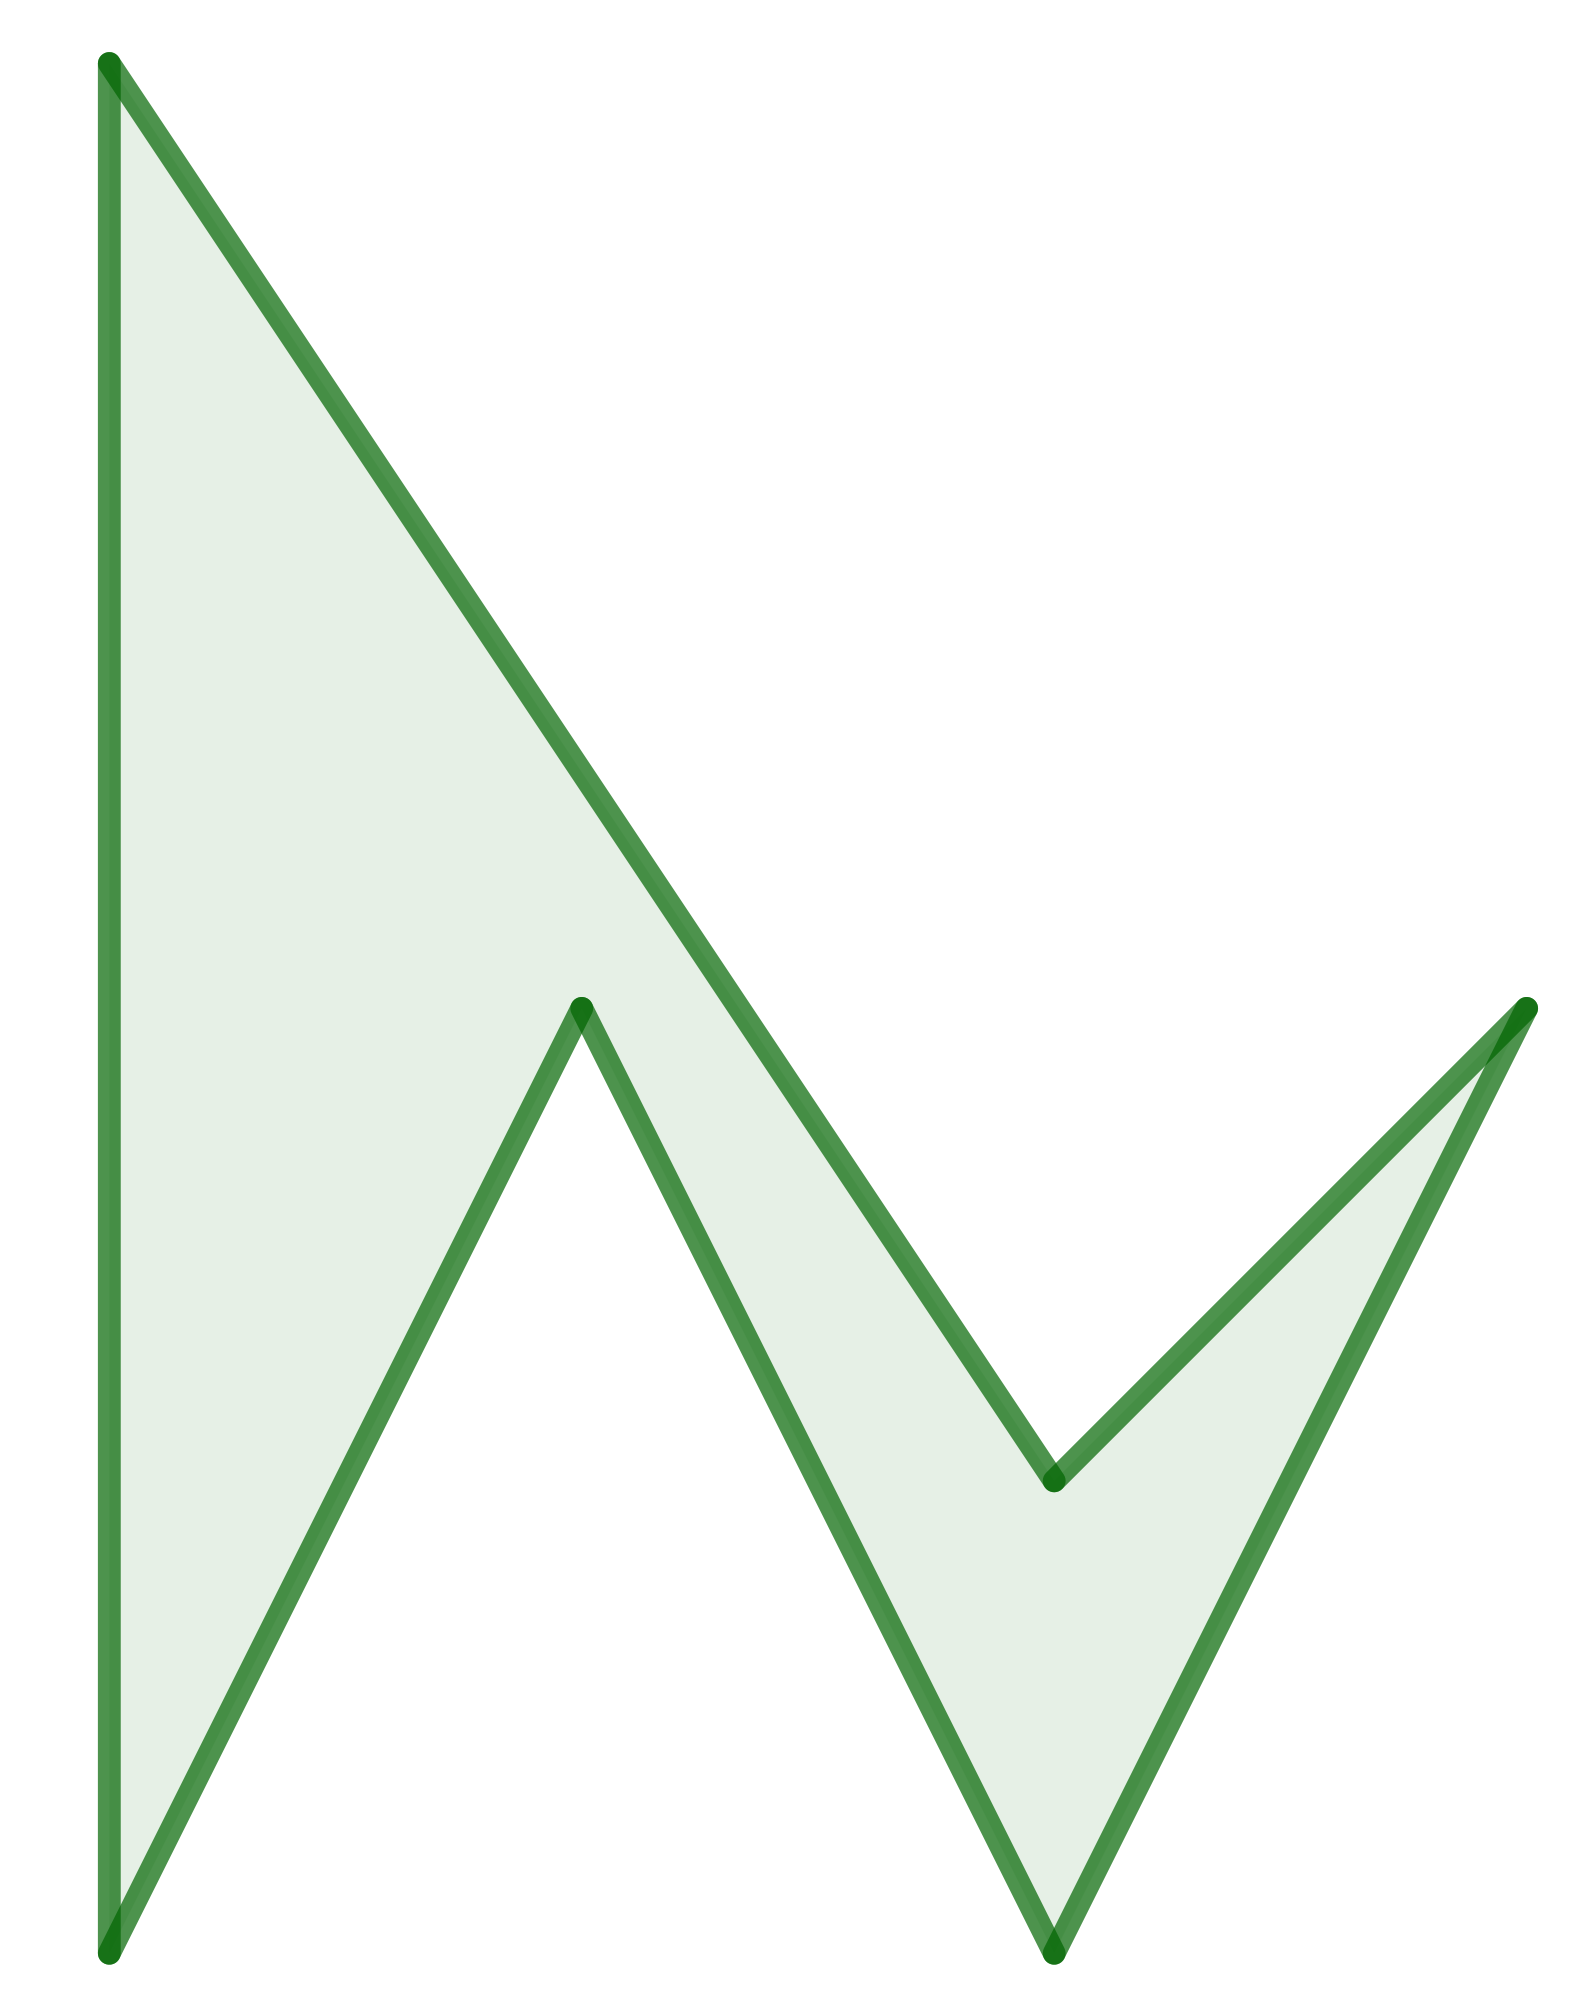
\includegraphics[scale=.4]{content/polygon/alg-area/mini-ear-1.png}

        	\smallskip
       		Un \ngone\ basique.
    	\end{center}

    	\begin{center}
        	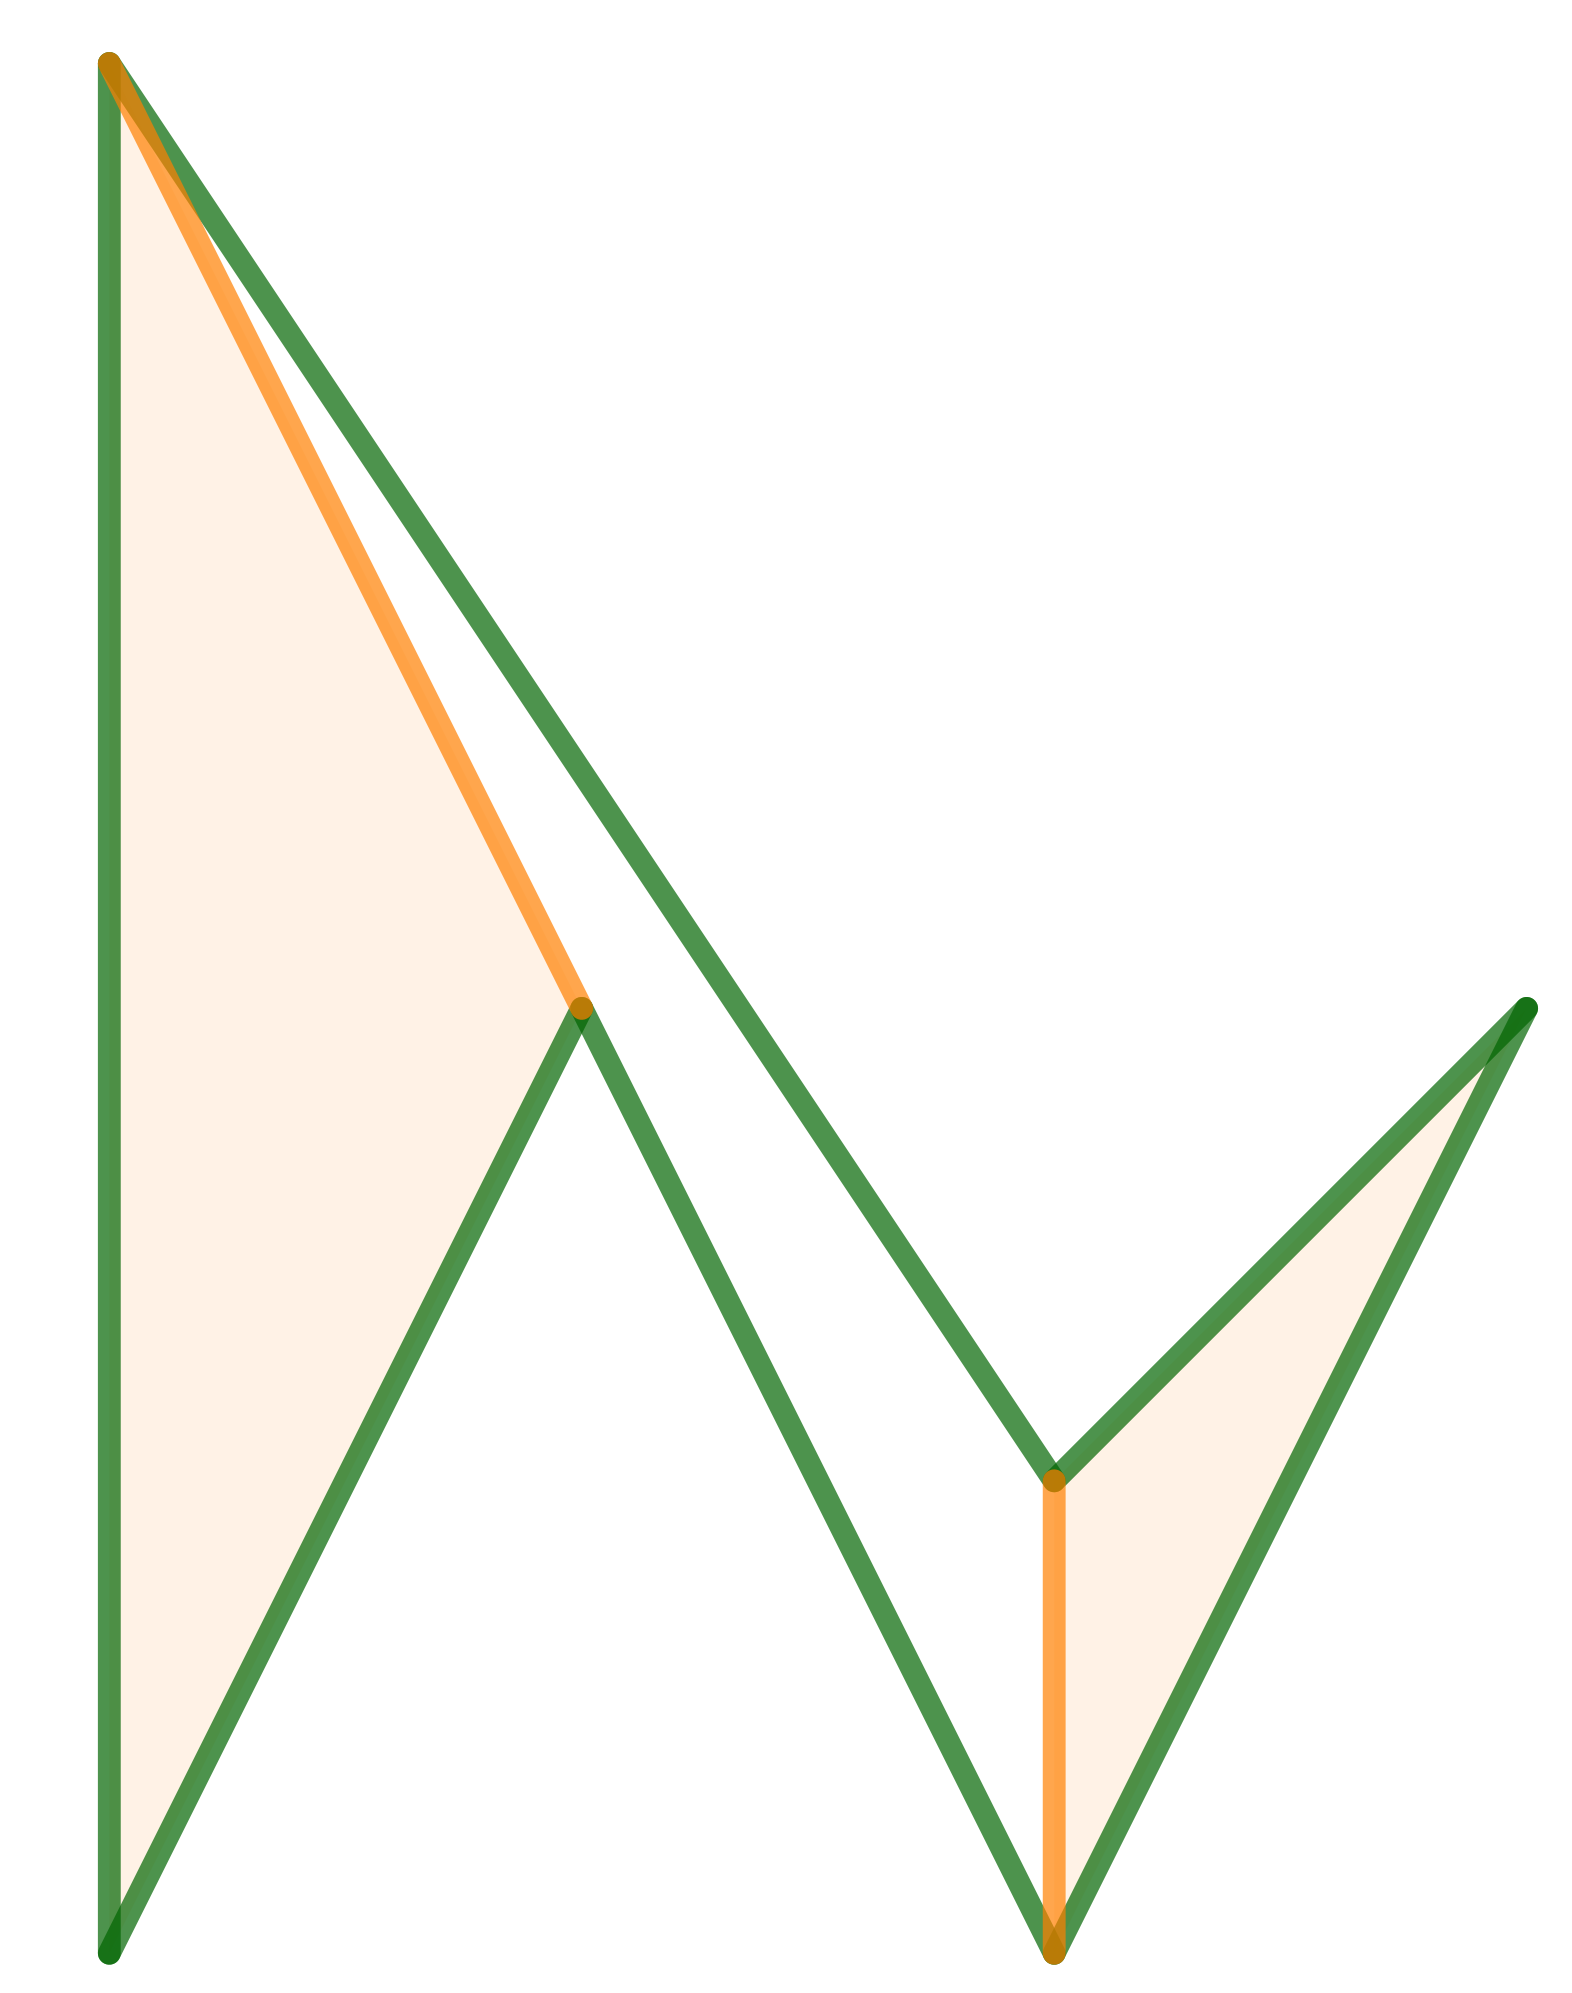
\includegraphics[scale=.4]{content/polygon/alg-area/mini-ear-2.png}

        	\smallskip
       		Juste deux oreilles disponibles.
    	\end{center}
    \end{multicols}


	Raisonnons donc par récurrence sur $n \in \NN_{\geq3}$.

	\begin{itemize}
		\item \textbf{Cas de base.}
		Soit $ABC$ un triangle. Dire que les sommets $A$, $B$ et $C$ sont parcourus dans le sens trigonométrique, c'est savoir que $\mu(ABC) = \det \big( \vect{AB} , \vect{AC} \big) > 0$.


		\item \textbf{Hérédité.}
		Soit un \ngone\ positif $\setproba{P} = A_1 A_2 \cdots A_n$ avec $n \in \NN_{>3}$. On peut supposer que $A_{n-1} A_n A_1$ est une oreille d'une triangulation à l'écoute du \ngone\ $\setproba{P}$.


	    \begin{multicols}{2}
    	    \small\itshape
    		\begin{center}
        	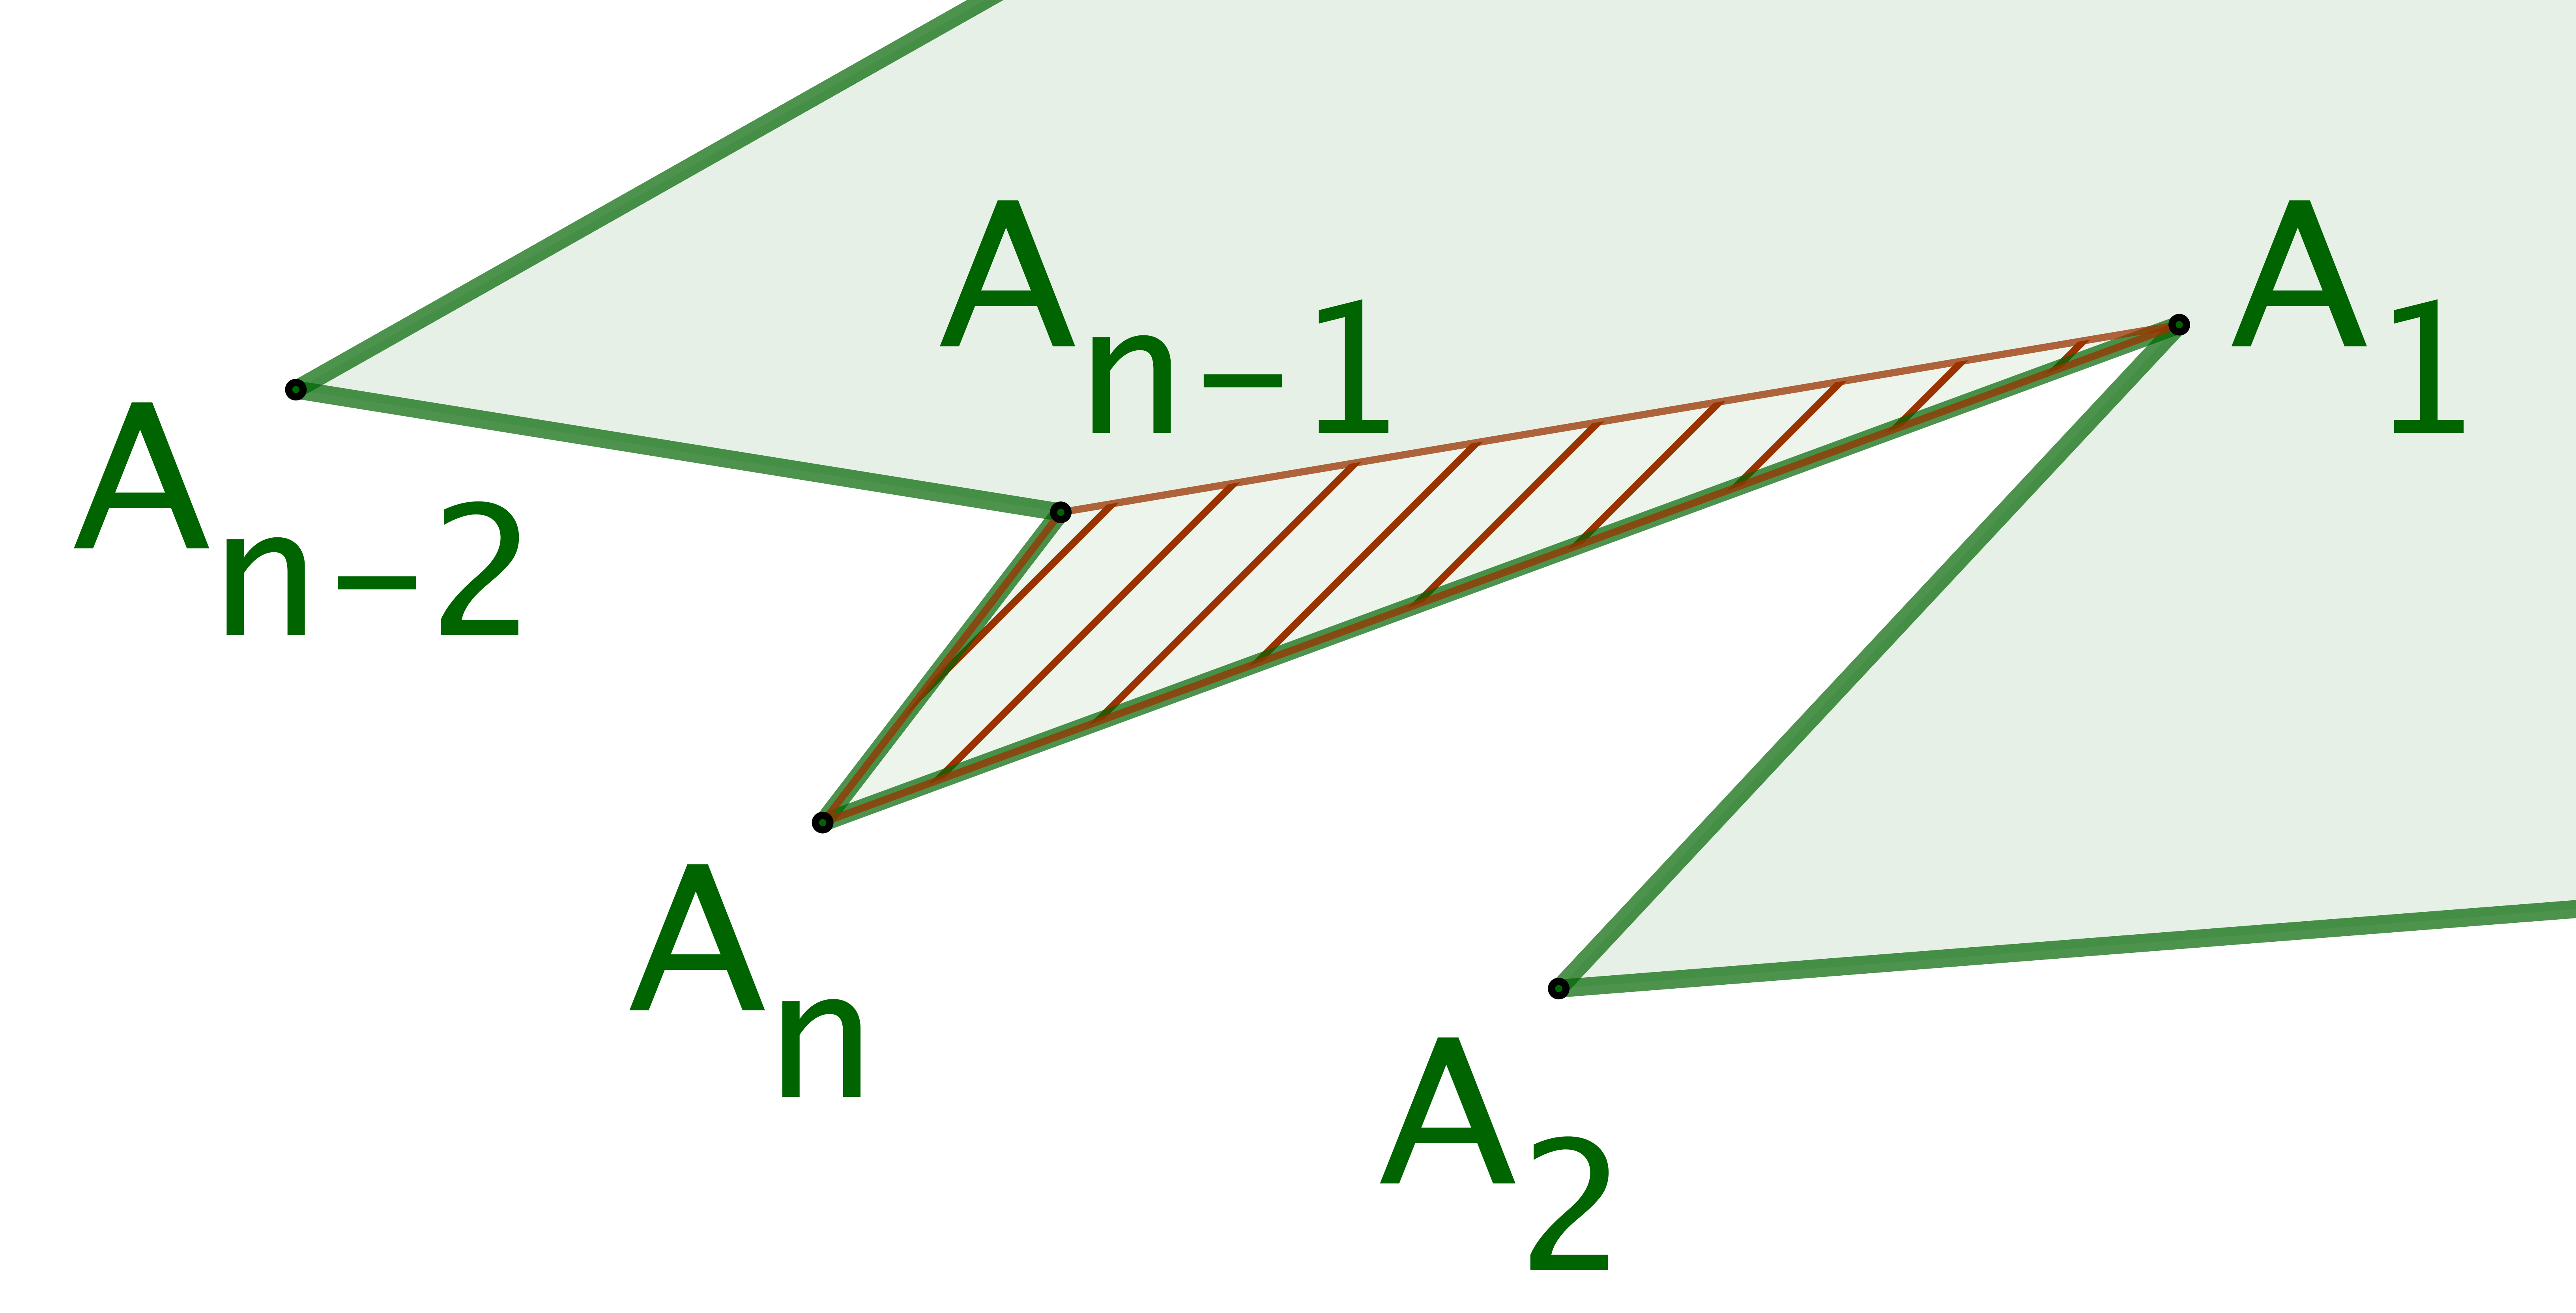
\includegraphics[scale=.4]{content/polygon/alg-area/triangulation-proof-OK.png}

	        	\smallskip
    	   		$A_{n-1} A_n A_1$ est une oreille.
    	\end{center}

	    	\begin{center}
        	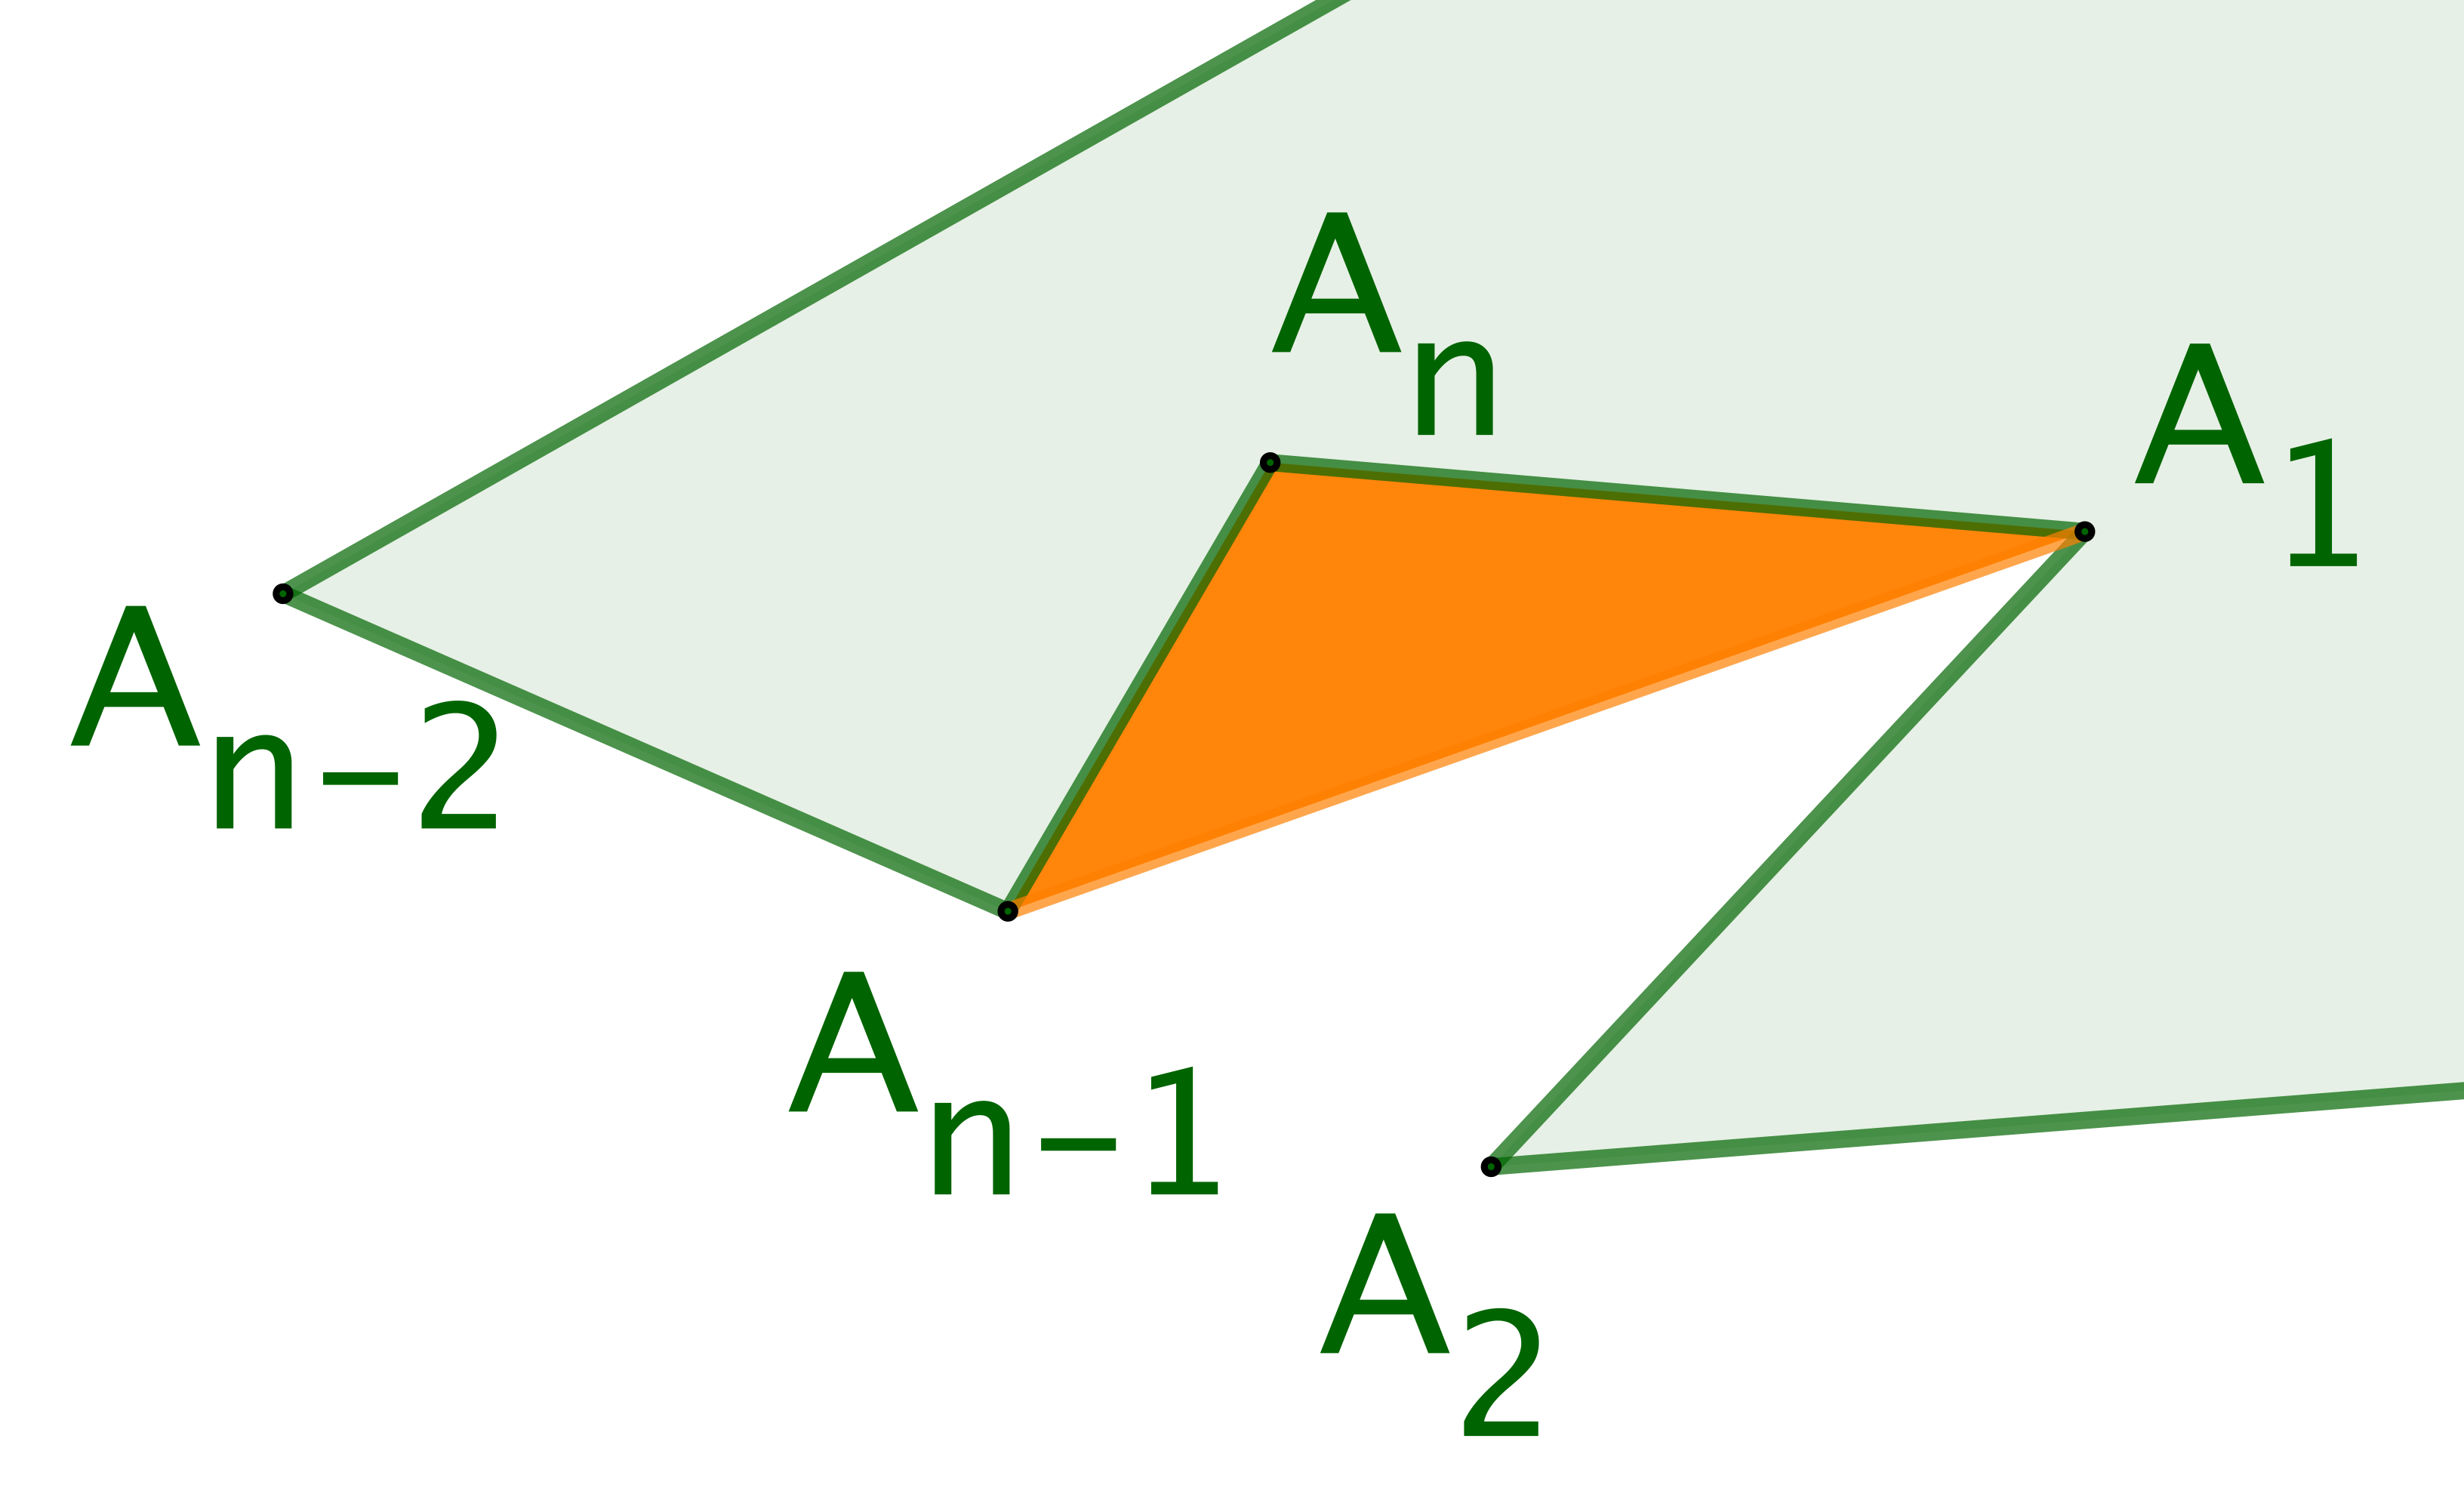
\includegraphics[scale=.4]{content/polygon/alg-area/triangulation-proof-KO.png}

        		\smallskip
    	   		$A_{n-1} A_n A_1$ n'est pas une oreille.
    		\end{center}
    	\end{multicols}


		\noindent
		Posons $\setproba{P}^{\,\prime} = A_1 \cdots A_{n-1}$ qui est positif comme $\setproba{P}$. 
		Nous arrivons aux calculs suivants en utilisant $A_1$ comme point de calcul de $\mu(\setproba{P})$.

		\leavevmode\kern-2em%
		\begin{stepcalc}[style=ar*]
			\mu(\setproba{P})
		%
%		\explnext{}
%			\dsum_{j=1}^{n} \det \big( \vect{A_1 \primeit{A}_j} , \vect{A_1 \primeit{A}_{j + 1}} \big)
%		%
		\explnext{}
			\dsum_{j=1}^{n} \det \big( \vect{A_1 \primeit{A}_j} , \vect{A_1 \primeit{A}_{j + 1}} \big)
%			+
%			\det \big( \vect{A_1 \primeit{A}_n} , \vect{A_1 \primeit{A}_{n+1}} \big)
		%
		\explnext*{$\primeit{A}_{n+1} = A_1$ \\
		           $\primeit{A}_i = A_i$ pour $i \leq n$}%
		          {}
			\dsum_{j=1}^{n-1} \det \big( \vect{A_1 A_j} , \vect{A_1 A_{j + 1}} \big)
%			+
%			\det \big( \vect{A_1 A_n} , \vect{A_1 A_1} \big)
		%
		\explnext{}
			\dsum_{j=1}^{n-2} \det \big( \vect{A_1 A_j} , \vect{A_1 A_{j + 1}} \big)
			+
			\det \big( \vect{A_1 A_{n-1}} , \vect{A_1 A_n} \big)
		%
		\explnext*{Pour $\mu(\setproba{P}^{\,\prime})$, noter que 
		        \\ $\det \big( \vect{A_1 A_{n-1}} , \vect{A_1 A_1} \big) = 0$.}{}
			\mu(\setproba{P}^{\,\prime})
			+
			\mu(A_{n-1} A_n A_1)
		\end{stepcalc}


		\noindent
		Par hypothèse de récurrence, nous savons que
		$\mu(\setproba{P}^{\,\prime}) \geq 0$.
		De plus, $A_{n-1} A_n A_1$ étant une oreille de $\setproba{P}$, 
		ce \xcycle{3} est forcément positif, d'où $\mu(A_{n-1} A_n A_1) \geq 0$ d'après le cas de base.
		Nous arrivons bien à $\mu(\setproba{P}) \geq 0$, ce qui permet de finir aisément la démonstration par récurrence.
	\end{itemize}
	
	\null\vspace{-6ex}
\end{proof}


% ----------------------- %


Le fait suivant nous montre que, pour les \ngones, l'aire algébrique est une extension de l'aire géométrique usuelle. Merci la tiangulisation!


\begin{fact} \label{sarea-ngone}
    Pour tout \ngone\ $\setproba{P}$, nous avons:
    $\area{\setproba{P}} = \abs{\sarea{\setproba{P}}}$.
\end{fact}


\begin{proof}
    Les deux points suivants permettent de faire une preuve par récurrence.

    \begin{itemize}
		\item \textbf{Cas de base.}
		L'égalité est immédiate pour les triangles (c'est ce qui a motivé la définition de l'aire algébrique).


		\item \textbf{Hérédité.}
		Soit $\setproba{P} = A_1 \cdots A_n$ un \ngone\ avec $n \in \NN_{>3}$.
		%
		Comme $\sarea{\setproba{P}^{\mathrm{op}}} = - \sarea{\setproba{P}}$ selon le fait \ref{nline-rota-opp}, nous pouvons choisir de parcourir $\setproba{P}$ positivement, puis de nous placer dans la situation de la démonstration du fait \ref{route-direction}:
		$A_{n-1} A_n A_1$ est une oreille positive d'une triangulation à l'écoute du \ngone\ $\setproba{P}$,
		et
		$\setproba{P}^{\,\prime} = A_1 \cdots A_{n-1}$ positif.
		%
		Nous arrivons alors aux calculs élémentaires suivants.
		
		\leavevmode\kern-2em%
		\begin{stepcalc}[style=ar*]
			\area{\setproba{P}}
		%
		\explnext*{$A_{n-1} A_n A_1$ est une oreille de $\setproba{P}$.}%
		          {}
		    \area{\setproba{P}^{\,\prime}} + \area{A_{n-1} A_n A_1}
		%
		\explnext*{Hypothèse de récurrence et cas de base.}%
		          {}
		    \frac12 \abs{\mu(\setproba{P}^{\,\prime})} + \frac12 \abs{\mu(A_{n-1} A_n A_1)}
		%
		\explnext*{Par positivité.}%
		          {}
		    \frac12 \big( \mu(\setproba{P}^{\,\prime}) + \mu(A_{n-1} A_n A_1) \big)
		%
		\explnext*{Comme dans la preuve du fait \ref{route-direction}.}%
		          {}
		    \frac12 \mu(\setproba{P})
		%
		\explnext*{Par positivité.}%
		          {}
		    \frac12 \abs{\mu(\setproba{P})}
		\explnext{}
		    \abs{\sarea{\setproba{P}}}
		\end{stepcalc}
    \end{itemize}
    
    \null\vspace{-3.5ex}
\end{proof}


% ----------------------- %


Finissons par un théorème de continuité qui permettra de justifier l'existence d'au moins une solution au problème d'isopérimétrie polygonale.


\begin{fact} \label{sarea-cont}
    Soient $n \in \NN_{\geq3}$ et
    $\pvaxes{O | i | j}$ un repère orthonormé direct du plan. 
    On note $\setproba{U} \subset \RR^{2n}$ l'ensemble des uplets de coordonnées $\big( x(A_1) ; y(A_1) ; \dots ; x(A_n) ; y(A_n) \big)$ où $A_1 A_2 \cdots A_n$ désigne un \ncycle,
    et $\alpha: \setproba{U} \rightarrow \RRp$ la fonction qui à un uplet de $\setproba{U}$ associe l'aire algébrique du \ncycle\ qu'il représente.
   	%
	Avec ces notations, la fonction $\alpha: \setproba{U} \rightarrow \RRp$ est continue.
\end{fact}


\begin{proof}
	Immédiat, car nous avons une fonction polynomiale.
\end{proof}
